\documentclass{article}

\usepackage[T1]{fontenc}
\usepackage[utf8]{inputenc}
\usepackage[brazilian]{babel}
\usepackage{graphicx}
\usepackage[export]{adjustbox}[2011/08/13]
\usepackage{float}
\usepackage[pdftex]{hyperref}
\usepackage{epstopdf}
\usepackage{etoolbox}
\usepackage{amsmath}
\usepackage{amsfonts}
\usepackage{amssymb}
\usepackage{caption}
\usepackage{subcaption}
\usepackage{setspace}
\usepackage{tikz}
\usepackage{listings}
\usepackage{xcolor} 

\bibliographystyle{eric}
\patchcmd{\thebibliography}{\section*}{\section}{}{}


\newcommand{\R}{\ensuremath{\mathbb{R}}}
\newcommand{\Prob}{\ensuremath{\mathbb{P}}}
\newcommand{\K}{\ensuremath{\mathbb{K}}}
\newcommand{\U}{\ensuremath{\mathbb{U}}}
\newcommand{\N}{\ensuremath{\mathbb{N}}}
\newcommand{\Lg}{\ensuremath{\mathbb{L}}}
\newcommand{\T}{\ensuremath{\rm Tr}}
\newcommand{\sg}{{\sigma(x_k)}}

\newcommand{\G}{\ensuremath{\mathcal{G}}}
\newcommand{\F}{\ensuremath{\mathcal{F}}}
\newcommand{\C}{\ensuremath{\mathcal{C}}}
\newcommand{\E}{\ensuremath{\mathcal{E}}}
\newcommand{\Hn}{\ensuremath{\mathcal{H}}}
\newcommand{\Hoo}{\ensuremath{\mathcal{H}_\infty}}
\newcommand{\Hop}{\ensuremath{\mathcal{H}_{op}}}
% --------------------------------------------------
\newtheorem{theo}{Teorema}
\newtheorem{exa}{Exemplo}
\newtheorem{lemm}{Lema}
\newtheorem{coro}{Corolário}
\newtheorem{defn}{Definição}[section]

\begin{document}
\input{capa.tex}

\onehalfspacing
\section{Objetivos}
	Este projeto tem como objetivo realizar o acionamento de um motor DC utilizando conversor de potência, controlar a posição por meio de servo-acionamento, e integrar componentes elétricos e mecânicos por malha de controle. 

\section{Motor e Conversor de Potência}
Implementamos no Simulink o circuito apresentado na figura \ref{fig:sim1}. Configuramos o bloco do motor DC disponível para que atuasse como motor DC de ímãs permanentes. Definimos os parâmetros do motor conforme especificado na tabela \ref{tab:param}. Determinamos o torque nominal do motor utilizando a equação \ref{eq:torque} e a constante de torque/corrente de armadura nominal resolvendo as equações \ref{eq:m1} e \ref{eq:m2}. Existem duas combinações possíveis de constante de torque e corrente nominal que atingem os pré requisitos, escolhemos a menor corrente.

\begin{equation}
	\label{eq:torque}
	T_{nom} = \frac{P_{nom}}{\omega_{nom}}
\end{equation}

\begin{equation}
\label{eq:m1}
	V_{nom} = R_a*I_{nom} + k_t*\omega_{nom}
\end{equation}

\begin{equation}
	\label{eq:m2}
	T_{nom} = k_t*I_{nom}
\end{equation}


\begin{figure}[H]
	\centering
	\includegraphics[width=\linewidth]{matlab/sim1}
	\caption{Esquemático da simulação para dimensionamento do motor DC e conversor}
	\label{fig:sim1}
\end{figure}

\begin{table}[]
	\centering
	\caption{Parâmetros do motor DC}
	\label{tab:param}
	\begin{tabular}{|c|c|}
		\hline
		\textbf{Parâmetro}              & \textbf{Valor}                 \\ \hline
		Potência nominal                & $5\ HP$                        \\ \hline
		Velocidade nominal              & $1750\ rpm$                    \\ \hline
		Tensão nominal                  & $240\ V$                       \\ \hline
		Torque nominal					& $20.3455\ Nm$ \\ \hline
		Corrente nominal				& $19.7128\ A$ \\ \hline
		Resistência de armadura ($R_a$) & $2,58\ \Omega$                 \\ \hline
		Indutância de armadura ($L_a$)  & $28\ mH$                       \\ \hline
		Inércia ($J$)                   & $2,22 \times 10^{-2}\ kg\ m^2$ \\ \hline
		Atrito viscoso ($B$)            & $2,95 \times 10^{-3}\ N\ m\ s$ \\ \hline
		Constante de Torque ($k_t$)		& $1.0321\ Nm/A$ \\ \hline
	\end{tabular}
\end{table}

Para o acionamento do motor, utilizamos uma ponte H composta por MOSFETs, sendo que o circuito de acionamento funciona com a diferença de potencial entre sinal de controle ($v_{cont}$) e uma onda triangular ($v_{tri}$), com funcionamento explicado pela figura \ref{fig:ponte}. Para fins de simulação utilizamos $v_{cont}$ e $v_{tri}$ variando entre $0\ V$ e $100\ V$, mas este valor pode variar desde que atenda aos requisitos de acionamento do MOSFET.

\begin{figure}[H]
	\centering
	\begin{subfigure}[t]{0.45\textwidth}
		\includegraphics[width=\linewidth]{ponte1}
		\caption{Controle e onda triangular}
	\end{subfigure}
	\begin{subfigure}[t]{0.45\textwidth}
		\includegraphics[width=\linewidth]{ponte2}
		\caption{Duty cycle e tensão de saída}
	\end{subfigure}
	\caption{Esquema de funcionamento do circuito de controle da ponte H}	
	\label{fig:ponte}
\end{figure}

A fim de garantir um bom fator de forma na saída do conversor, colocamos um capacitor de filtro $C_f$ em paralelo com a carga. Para o motor em questão chegamos ao seguinte valor:

\begin{equation}
C_f=1000\ \mu F
\end{equation}

Fizemos a simulação da resposta do motor a um degrau com $V_{out}=240\ V$, sem cargas, apenas com os parâmetros físicos definidos nele mesmo.
Obtivemos os resultados de tensão e correntes de armadura ($v_a$ e $i_a$), e também curvas de torque e velocidade angular ($T_{em}$ e $\omega_m$) conforme figura \ref{fig:sim1viwt}.

\begin{figure}[H]
	\centering
	\begin{subfigure}{0.45\textwidth}
		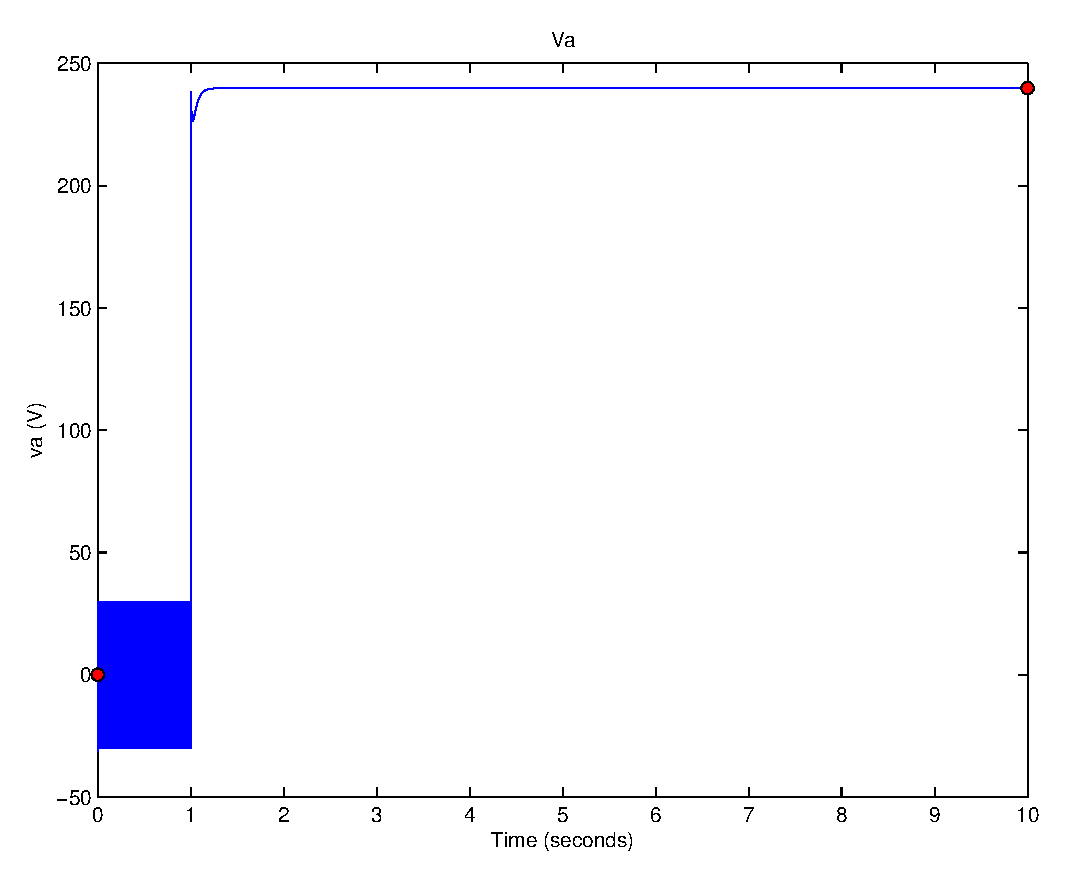
\includegraphics[width=\linewidth]{matlab/va1}
		\caption{Tensão de armadura}
	\end{subfigure}
	\begin{subfigure}{0.45\textwidth}
		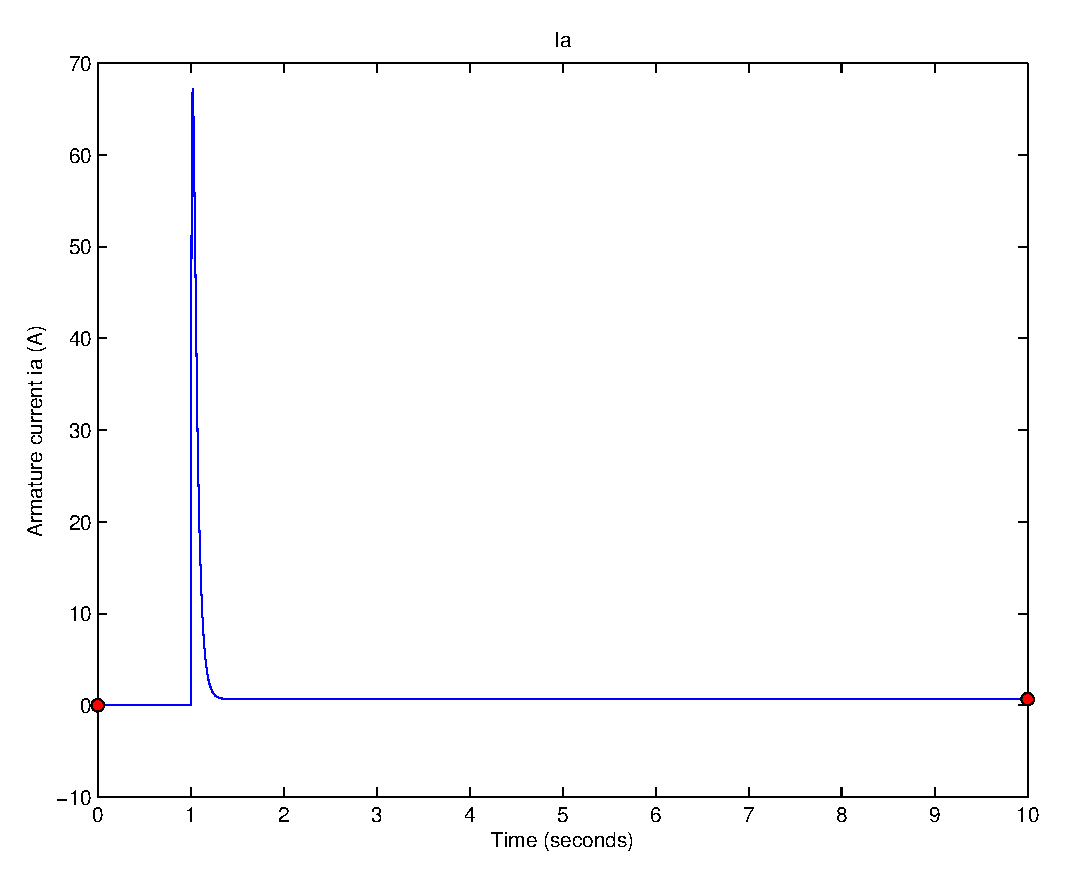
\includegraphics[width=\linewidth]{matlab/ia1}
		\caption{Corrente de armadura}
	\end{subfigure}
	\begin{subfigure}{0.45\textwidth}
		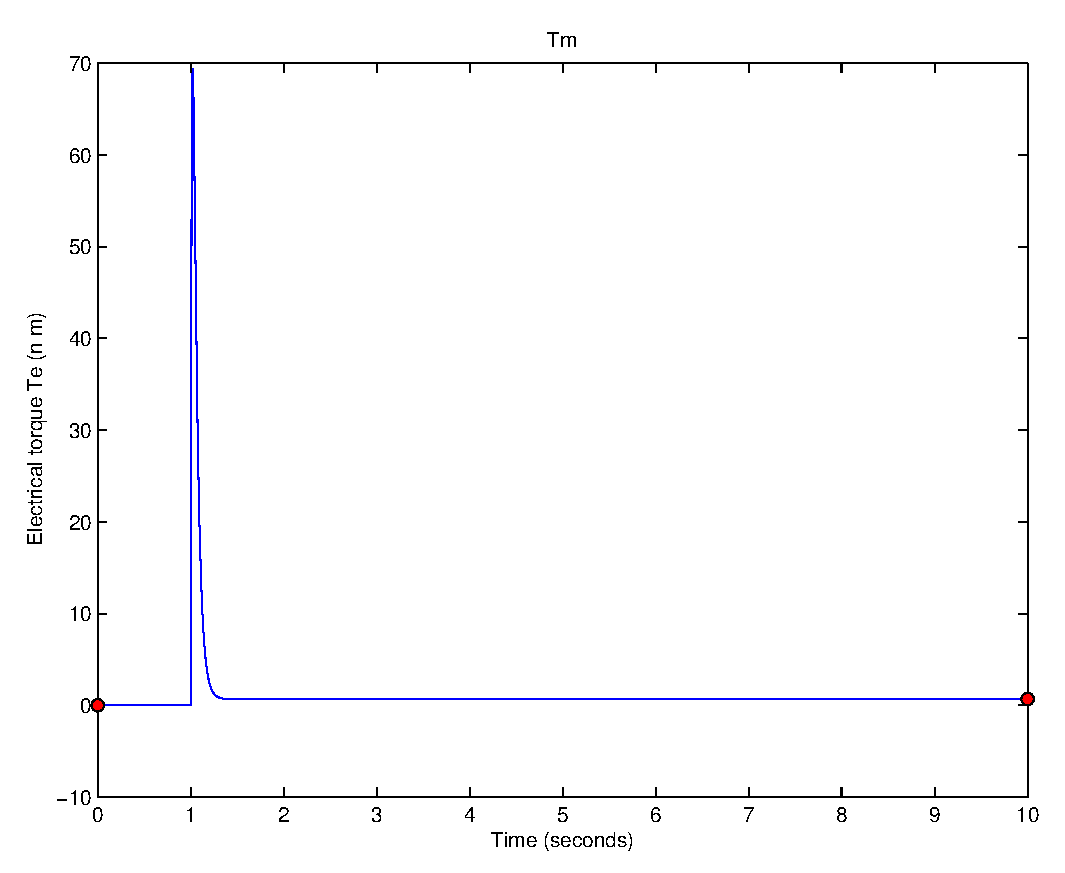
\includegraphics[width=\linewidth]{matlab/tm1}
		\caption{Torque}
	\end{subfigure}
	\begin{subfigure}{0.45\textwidth}
		\includegraphics[width=\linewidth]{matlab/wm1}
		\caption{Velocidade angular}
	\end{subfigure}
	\caption{Resposta ao degrau de $240\ V$ no motor DC}	
	\label{fig:sim1viwt}
\end{figure}

Podemos ver que ainda existe uma oscilação significativa na tensão de armadura, porém julgamos inviável aumentar a capacitância de filtro. Notamos também que a velocidade atingida supera a velocidade nominal, fator esperado uma vez que estamos trabalhando sem carga. Existe um pico de corrente que ultrapassa significativamente o valor nominal e que pode vir a danificar o motor.

\section{Servo-acionamento}
Iniciamos o projeto do servo-acionamento pelo controle PI de corrente. Utilizando o Simulink, conforme figura \ref{fig:sim2}.

\begin{figure}[H]
	\centering
	\includegraphics[width=\linewidth]{matlab/sim2}
	\caption{Esquemático da simulação do controlador de corrente}
	\label{fig:sim2}
\end{figure}

Para facilitar o controle somamos um offset de $50\%$ no duty-cycle de saída, assim se o esforço de controle for negativo a tensão sobre o motor será negativa e se este for positivo a tensão será positiva. Dimensionamos o controlador PI para que ele responda a um degrau unitário com erro estacionário de menos de $0,2\ A$ e com tempo de resposta menor do que $100\ ms$. Para isso escolhemos as constantes proporcional e integral de maneira iterativa, ajustando-as de para atingir nosso objetivo. As constantes escolhidas foram:
\begin{equation}
	k_p = 3
\end{equation}
\begin{equation}
	k_i = 100
\end{equation}

A resposta do controlador ao degrau unitário está apresentada na figura \ref{fig:ia2}, podemos ver que ele tem uma resposta satisfatória considerando os requisitos de projeto.
\begin{figure}[H]
	\centering
	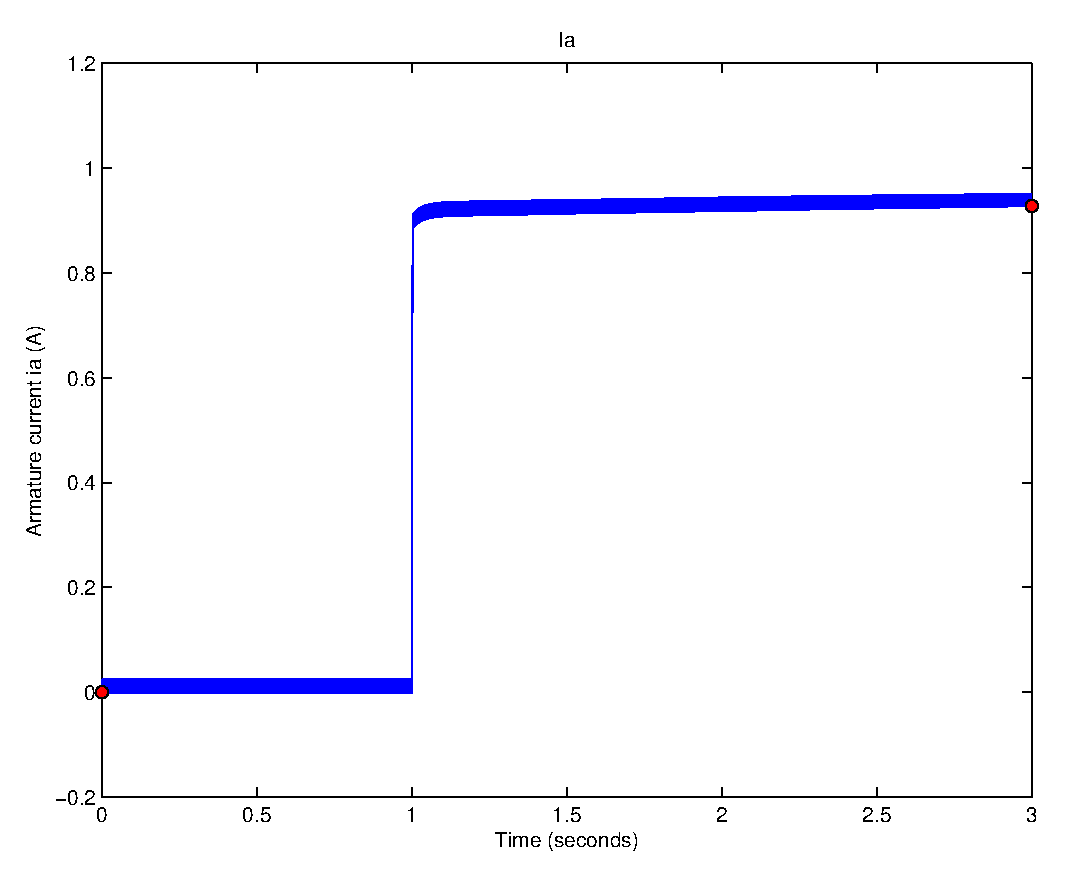
\includegraphics[width=0.7\linewidth]{matlab/ia2}
	\caption{Resposta do controlador de corrente ao degrau unitário}
	\label{fig:ia2}
\end{figure}

Projetamos então um controlador PI para a velocidade angular do motor, cuja saída é saturada no valor de corrente nominal e serve de referência para nosso controlador de corrente. O esquema desse sistema pode ser visto na figura \ref{fig:sim3}.

\begin{figure}[H]
	\centering
	\includegraphics[width=\linewidth]{matlab/sim3}
	\caption{Esquemático da simulação do controlador de velocidade}
	\label{fig:sim3}
\end{figure}

Projetamos esse controlador para que ele possua um erro estacionário de menos do que $0.2\ rad/s$ com tempo de resposta menor do que $400\ ms$. Para isso encontramos as constantes:
\begin{equation}
	k_p = 10
\end{equation}
\begin{equation}
	k_i = 1
\end{equation}
Simulamos a resposta do controlador a um degrau de velocidade de $100\ rad/s$ para um motor sem carga, encontrando os resultados apresentados na figura \ref{fig:sim3viwt}. Podemos ver que novamente o controlador cumpre os requisitos do projeto e que o problema do pico de corrente no motor foi resolvido.

\begin{figure}[H]
	\centering
	\begin{subfigure}{0.45\textwidth}
		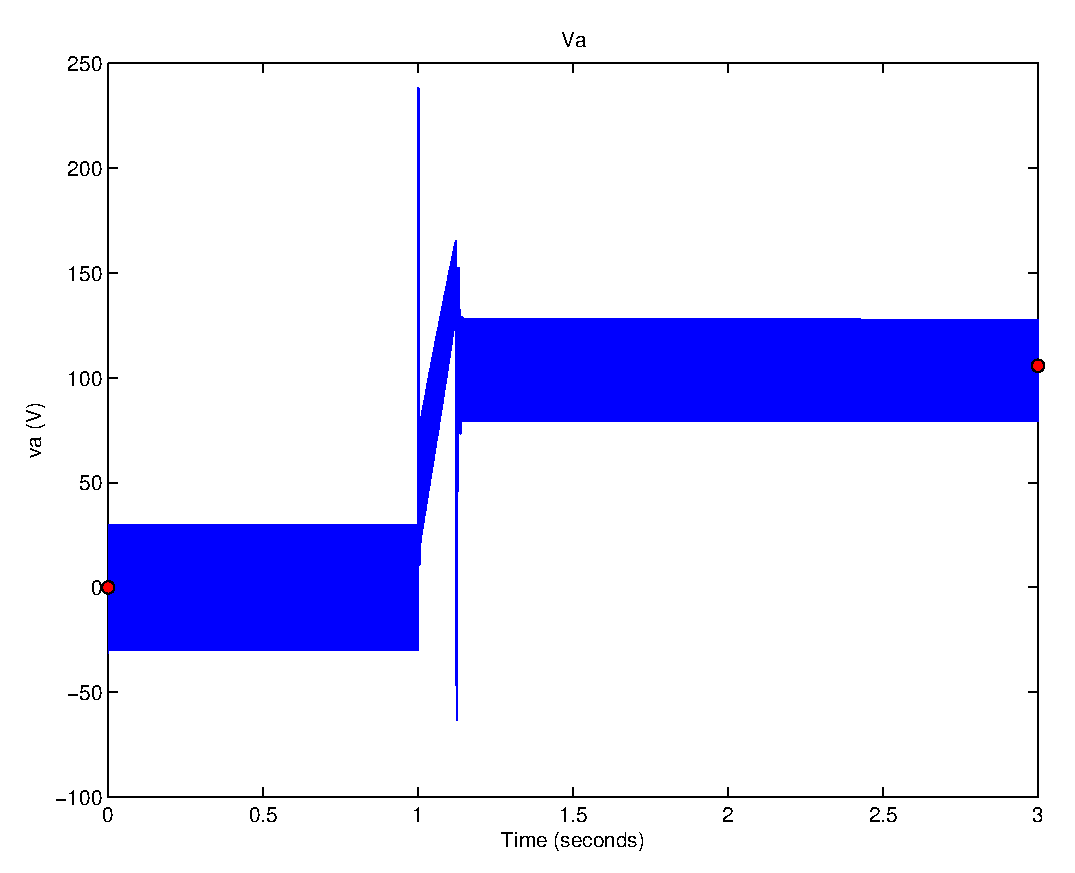
\includegraphics[width=\linewidth]{matlab/va3}
		\caption{Tensão de armadura}
	\end{subfigure}
	\begin{subfigure}{0.45\textwidth}
		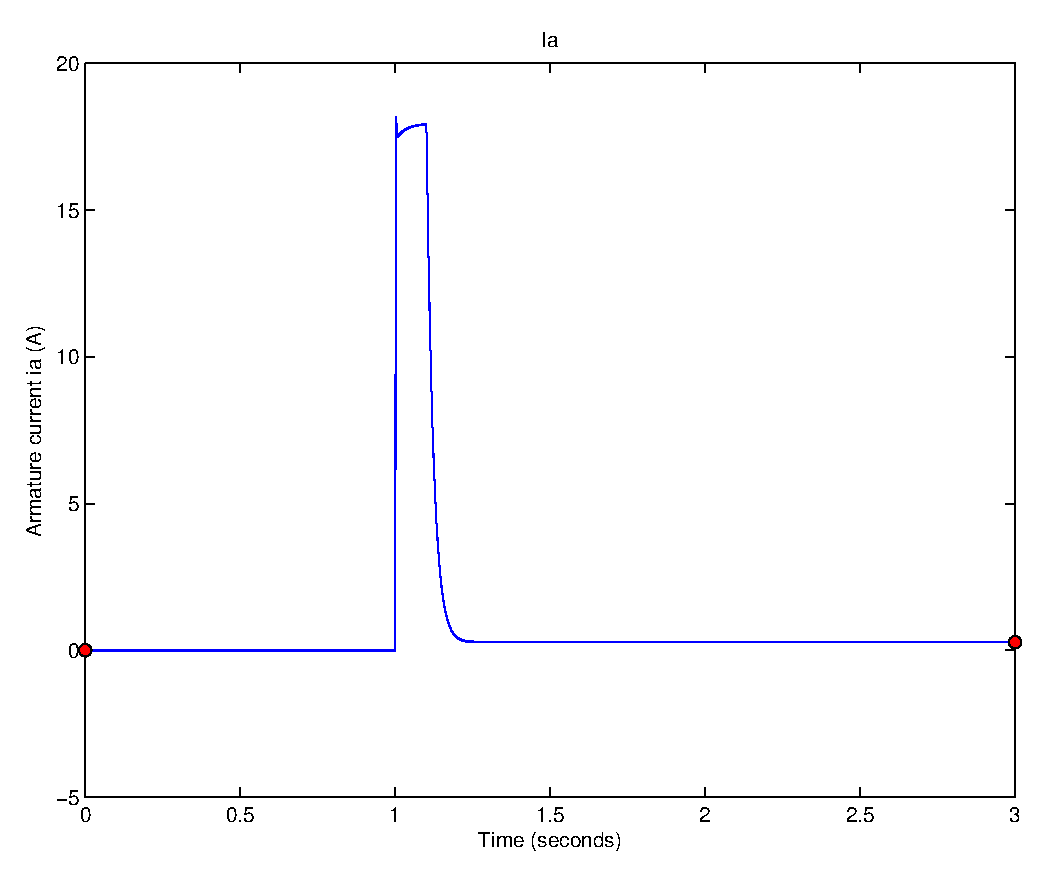
\includegraphics[width=\linewidth]{matlab/ia3}
		\caption{Corrente de armadura}
	\end{subfigure}
	\begin{subfigure}{0.45\textwidth}
		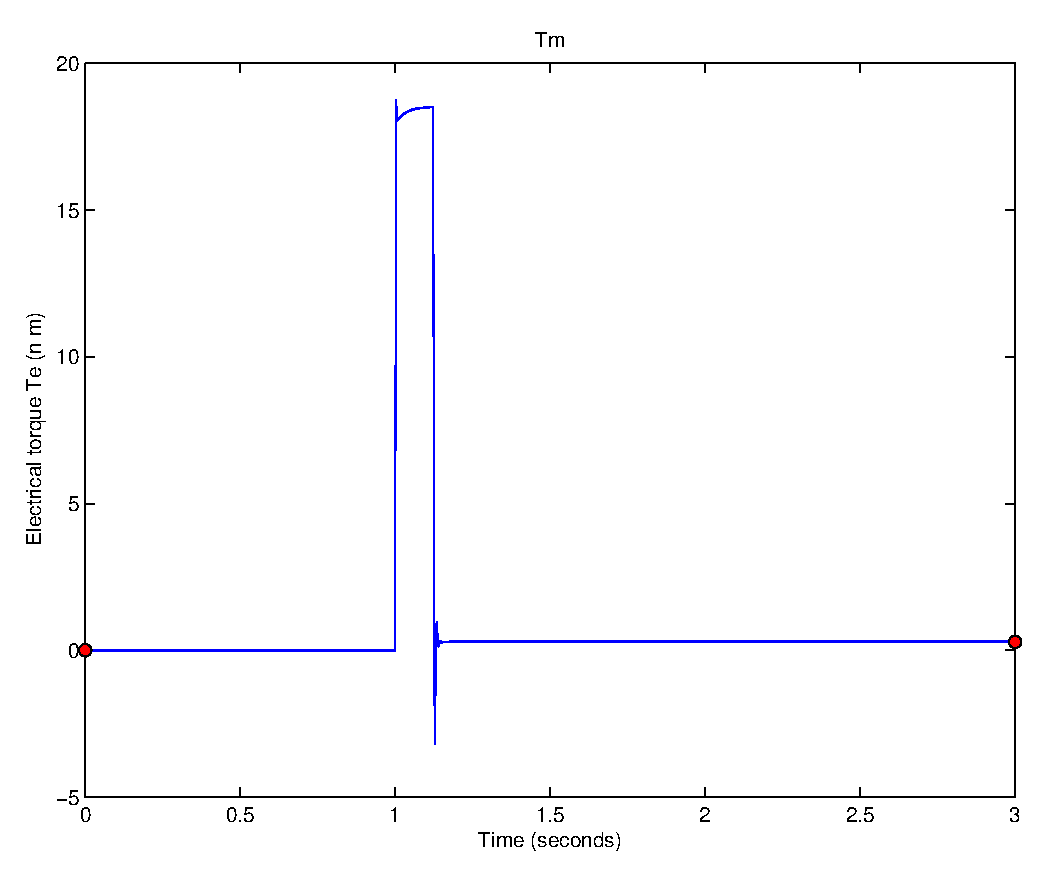
\includegraphics[width=\linewidth]{matlab/tm3}
		\caption{Torque}
	\end{subfigure}
	\begin{subfigure}{0.45\textwidth}
		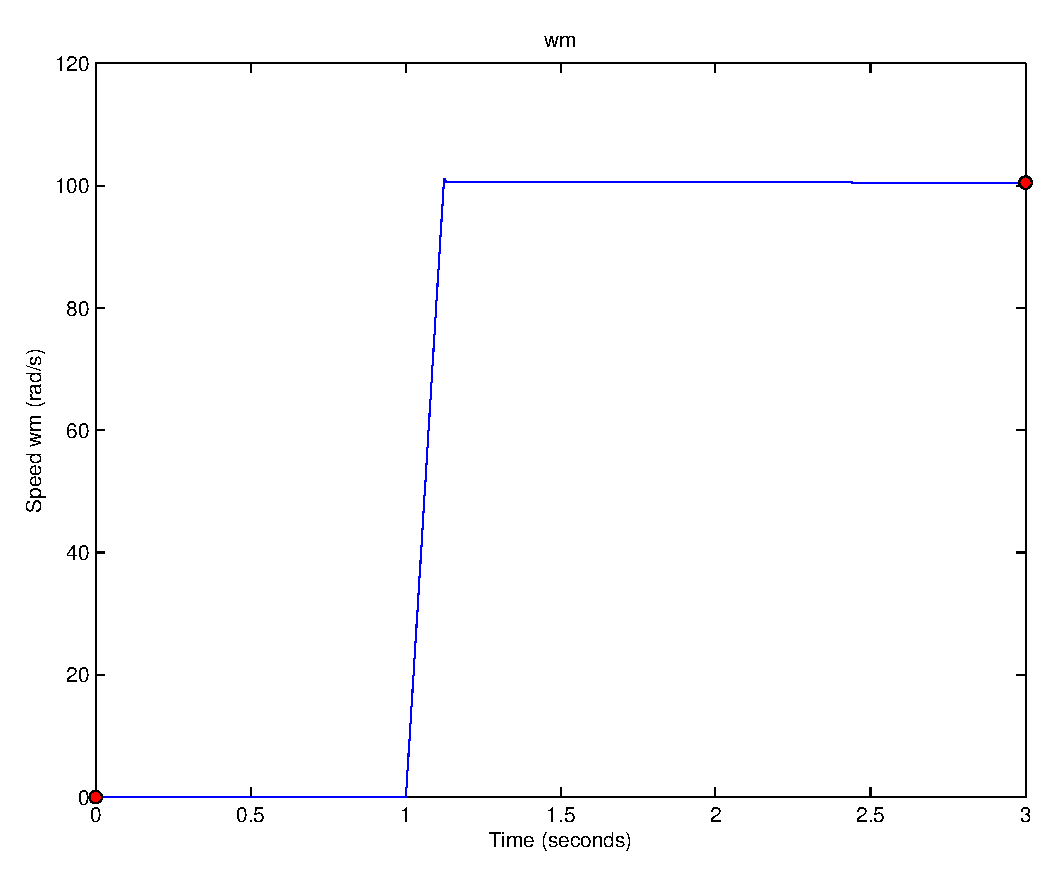
\includegraphics[width=\linewidth]{matlab/wm3}
		\caption{Velocidade angular}
	\end{subfigure}
	\caption{Resposta ao degrau de $100\ rad/s$ para controlador de velocidade}	
	\label{fig:sim3viwt}
\end{figure}

O dimensionamento dos ganhos de ambos controladores seguiram o mesmo procedimento, nós primeiro encontramos um valor para o ganho proporcional que atendia os pré requisitos de tempo de resposta e depois ajustamos a constante integral para controlar o erro estacionário.

\section{Modelagem do Manipulador}
Realizamos a modelagem mecânica do manipulador robótico simplificado, conforme especificado no roteiro. O sistema foi reduzido para uma junta rotacional cujo link tem massa $4\ kg$, comprimento $60\ cm$ e que atua em um range de $0$ à $90^\circ$, conforme apresentado na figura \ref{fig:robo}.

\begin{figure}[H]
	\centering
	\includegraphics[width=0.5\linewidth]{robo}
	\caption{Manipulador robótico de 1 grau de liberdade}
	\label{fig:robo}
\end{figure}

Encontramos o modelo cinemático direto notando que a posição (X,Y) da garra do robô é dada por:
\begin{equation}
	X(\theta) = d\cdot cos(\theta)
\end{equation}
\begin{equation}
	Y(\theta) = d\cdot sin(\theta)
\end{equation}

Podemos calcular o modelo cinemático inverso notando que:
\begin{equation}
	\theta(x,y) = atan(\frac{y}{x})
\end{equation}

Encontramos então o modelo dinâmico da junta, encontrando o torque nela dada uma posição e aceleração, para isso calculamos primeiramente o momento de inércia do link, obtendo:
\begin{equation}
	J_{link} = \frac{m\cdot d^2}{3}
\end{equation}
Calculamos então o torque gerado pela força peso, obtendo:
\begin{equation}
	\tau_{P}(\theta) = m\cdot g\cdot \frac{d\cdot cos(\theta)}{2}
\end{equation}
O modelo dinâmico pode então ser representado como:
\begin{equation}
	\tau(\theta, \ddot{\theta}) = m\cdot g\cdot \frac{d\cdot cos(\theta)}{2} + J_{link}\cdot \ddot{\theta}
\end{equation}
Para simplificar a simulação, consideramos que o torque da ferramenta é só causado pela força peso e somamos seu momento de inércia ao momento de inércia do motor. Simulamos a resposta do sistema para um perfil de velocidade trapezoidal com tempo de aceleração e desaceleração de $10\%$ do tempo do movimento que leva o robô da posição $\theta=0^\circ$ para $\theta=90^\circ$ em um, cinco e dez segundos. O esquema da simulação pode ser visto na figura \ref{fig:sim7} e os resultados na figuras \ref{fig:sim7res}, \ref{fig:sim8res} e \ref{fig:sim9res}.

\begin{figure}[H]
	\centering
	\includegraphics[width=\linewidth]{matlab/sim7}
	\caption{Esquemático da simulação do modelo dinâmico}
	\label{fig:sim7}
\end{figure}

\begin{figure}[H]
	\centering
	\begin{subfigure}{0.45\textwidth}
		\includegraphics[width=\linewidth]{matlab/theta7}
		\caption{Posição $\theta$}
	\end{subfigure}
	\begin{subfigure}{0.45\textwidth}
		\includegraphics[width=\linewidth]{matlab/y7}
		\caption{Posição Y}
	\end{subfigure}
	\begin{subfigure}{0.45\textwidth}
		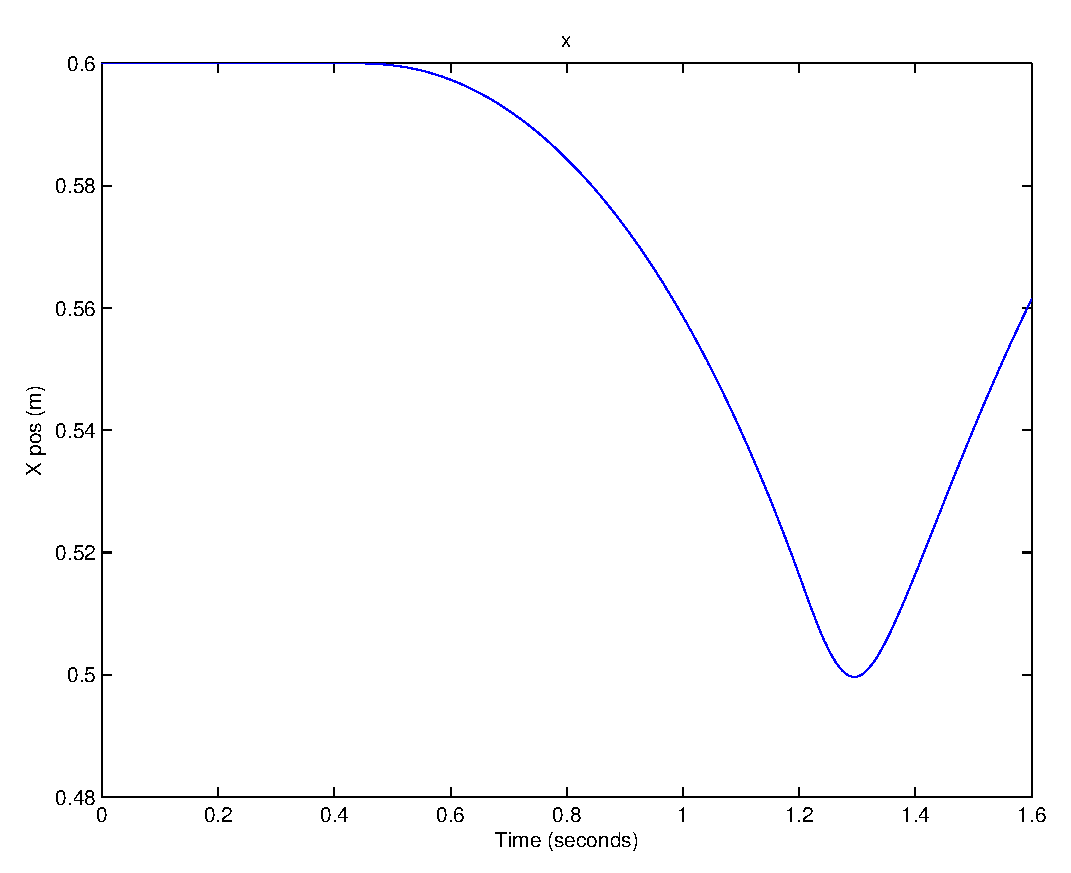
\includegraphics[width=\linewidth]{matlab/x7}
		\caption{Posição X}
	\end{subfigure}
	\begin{subfigure}{0.45\textwidth}
		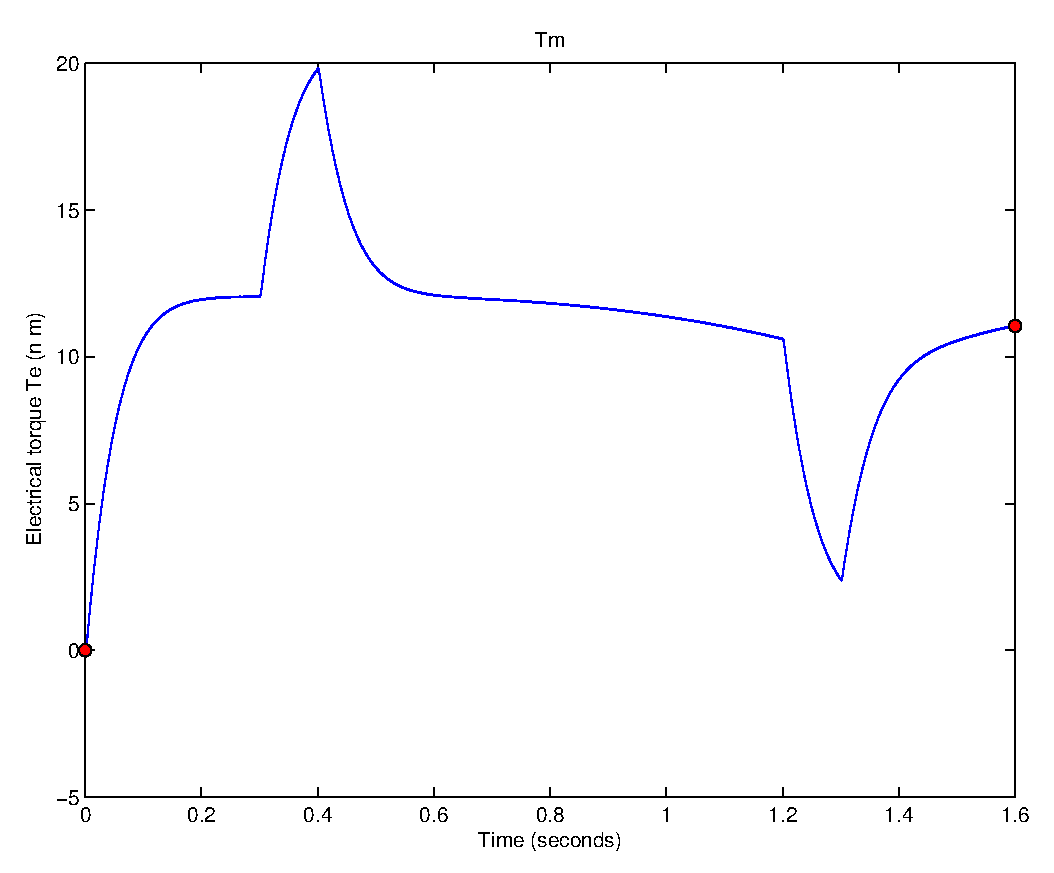
\includegraphics[width=\linewidth]{matlab/tm7}
		\caption{Torque}
	\end{subfigure}
	\begin{subfigure}{0.45\textwidth}
		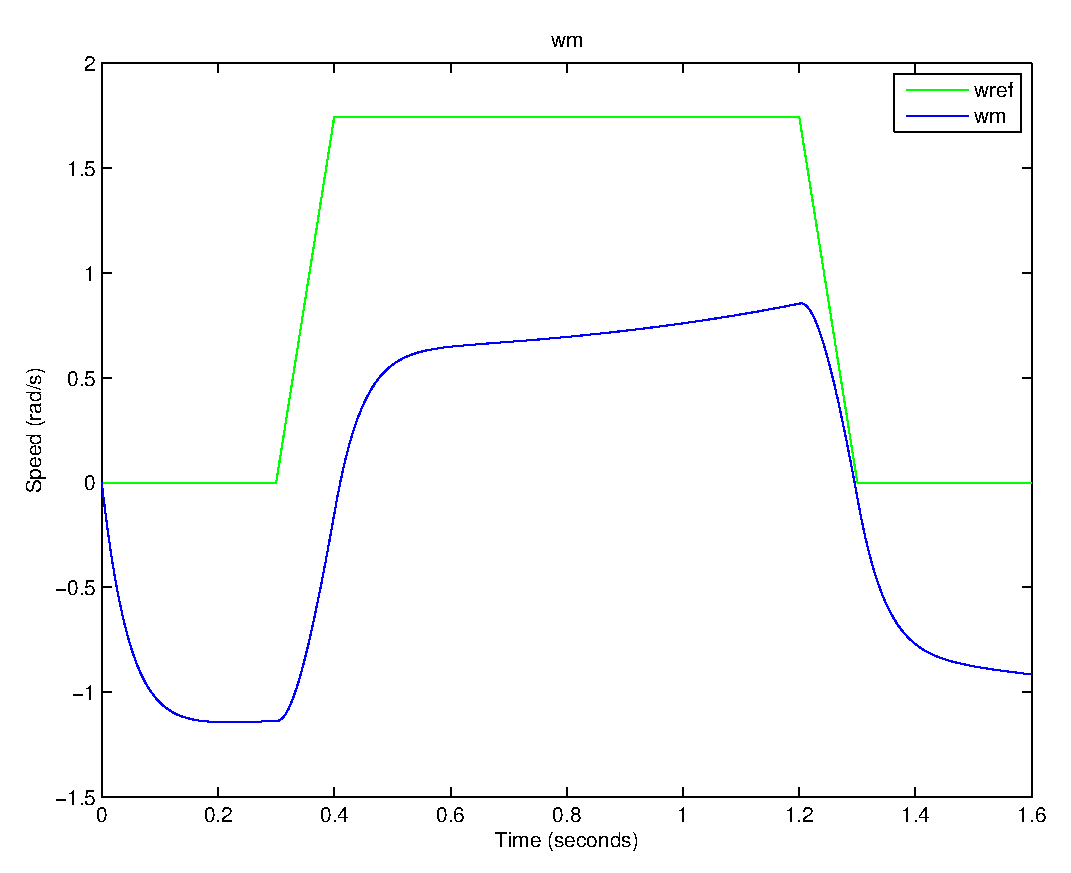
\includegraphics[width=\linewidth]{matlab/wm7}
		\caption{Velocidade angular}
	\end{subfigure}
	\caption{Resposta à perfil de velocidade trapezoidal de 1 segundo}	
	\label{fig:sim7res}
\end{figure}

\begin{figure}[H]
	\centering
	\begin{subfigure}{0.45\textwidth}
		\includegraphics[width=\linewidth]{matlab/theta8}
		\caption{Posição $\theta$}
	\end{subfigure}
	\begin{subfigure}{0.45\textwidth}
		\includegraphics[width=\linewidth]{matlab/y8}
		\caption{Posição Y}
	\end{subfigure}
	\begin{subfigure}{0.45\textwidth}
		\includegraphics[width=\linewidth]{matlab/x8}
		\caption{Posição X}
	\end{subfigure}
	\begin{subfigure}{0.45\textwidth}
		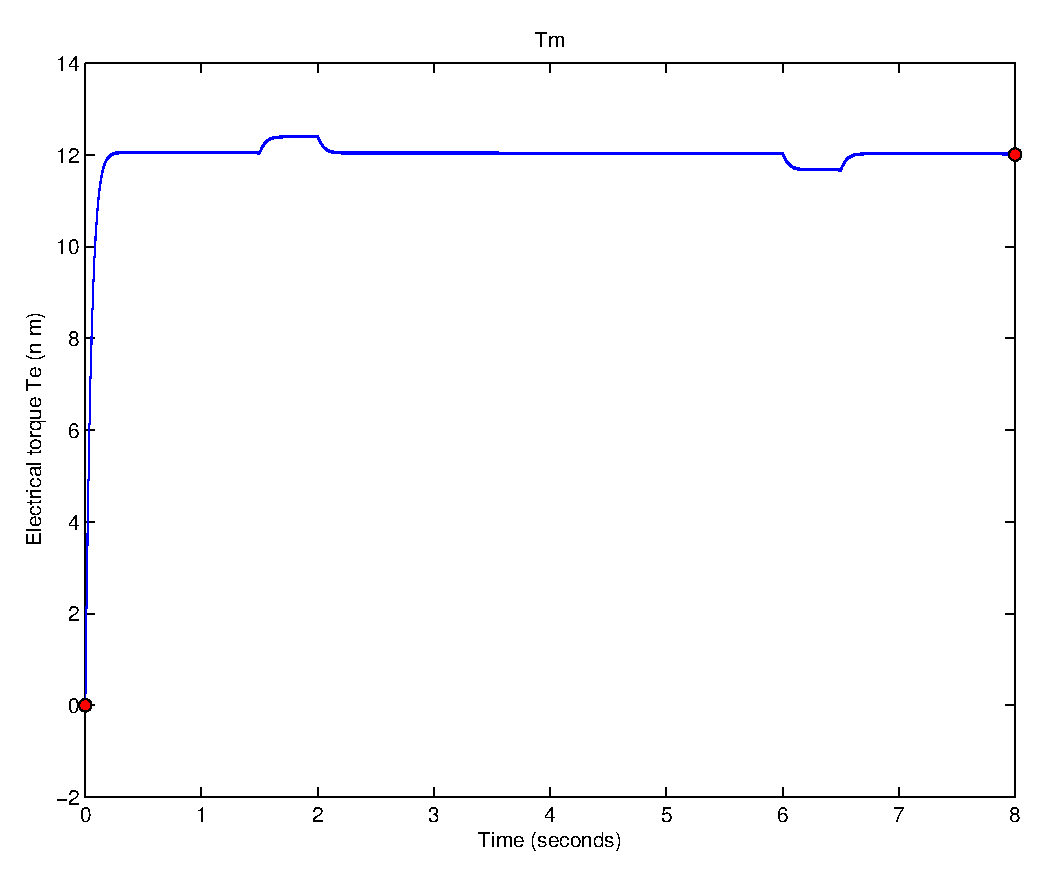
\includegraphics[width=\linewidth]{matlab/tm8}
		\caption{Torque}
	\end{subfigure}
	\begin{subfigure}{0.45\textwidth}
		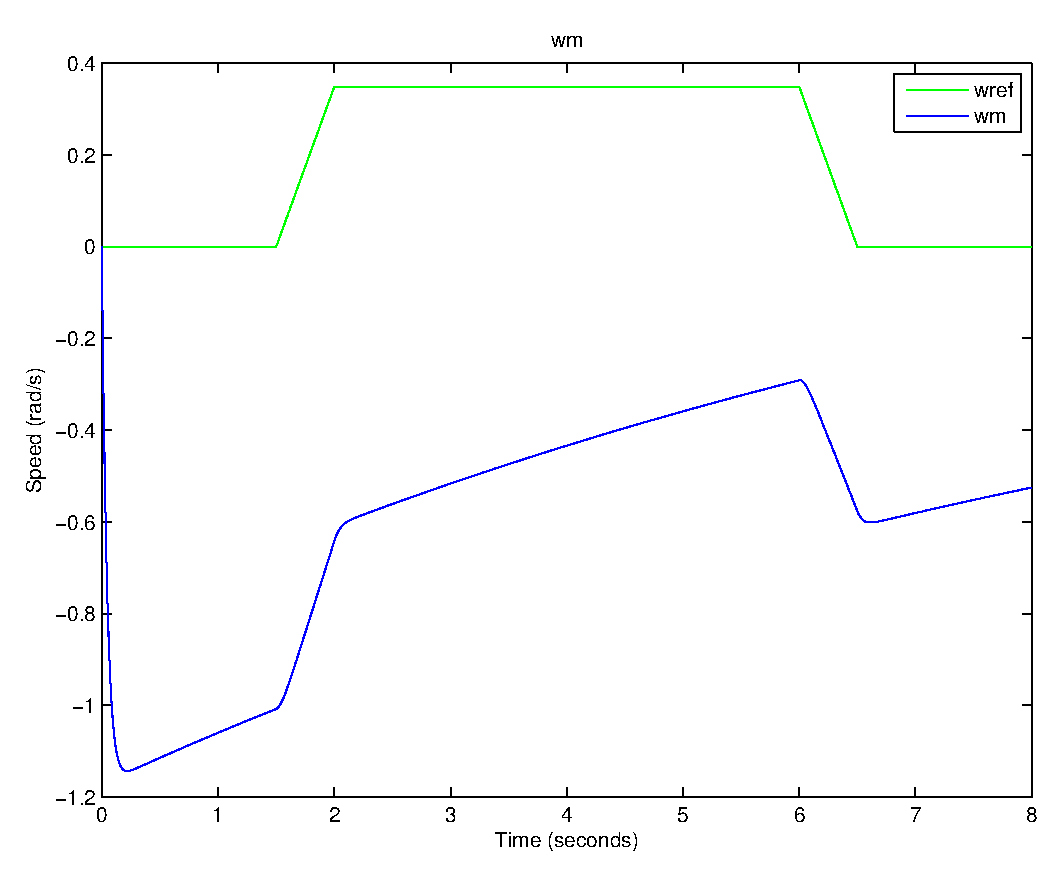
\includegraphics[width=\linewidth]{matlab/wm8}
		\caption{Velocidade angular}
	\end{subfigure}
	\caption{Resposta à perfil de velocidade trapezoidal de 5 segundos}	
	\label{fig:sim8res}
\end{figure}

\begin{figure}[H]
	\centering
	\begin{subfigure}{0.45\textwidth}
		\includegraphics[width=\linewidth]{matlab/theta9}
		\caption{Posição $\theta$}
	\end{subfigure}
	\begin{subfigure}{0.45\textwidth}
		\includegraphics[width=\linewidth]{matlab/y9}
		\caption{Posição Y}
	\end{subfigure}
	\begin{subfigure}{0.45\textwidth}
		\includegraphics[width=\linewidth]{matlab/x9}
		\caption{Posição X}
	\end{subfigure}
	\begin{subfigure}{0.45\textwidth}
		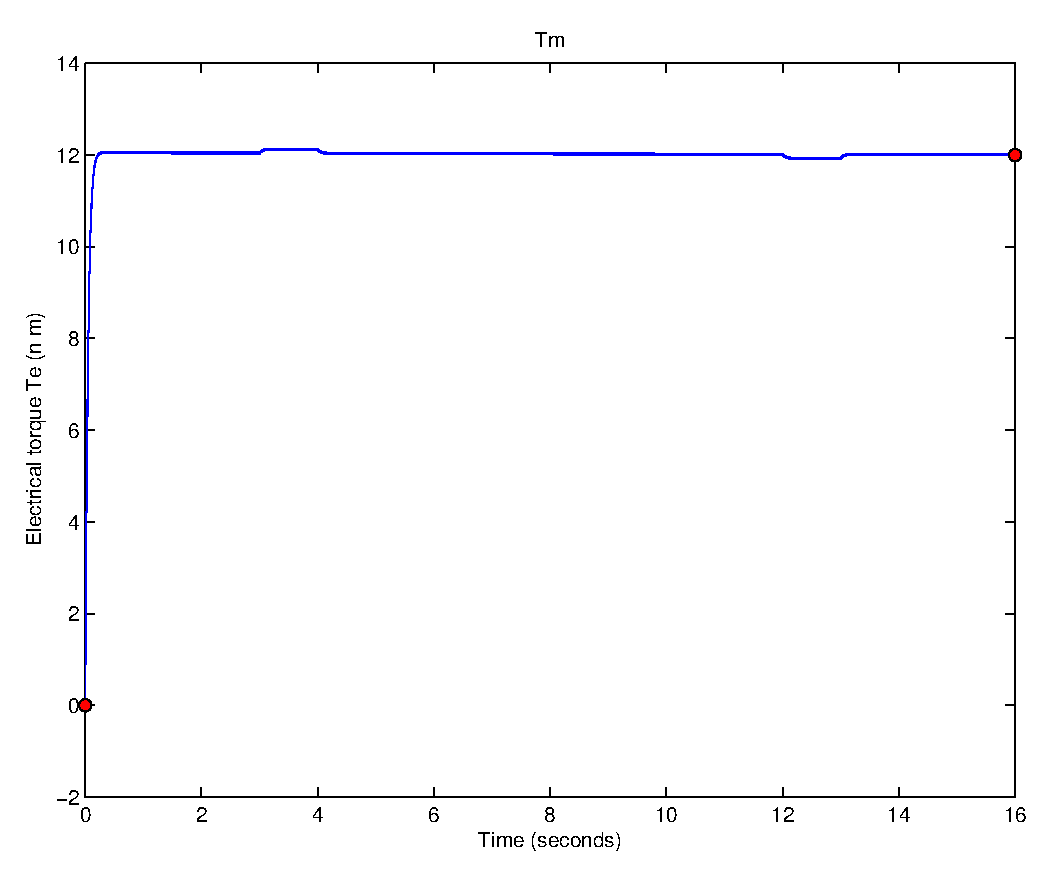
\includegraphics[width=\linewidth]{matlab/tm9}
		\caption{Torque}
	\end{subfigure}
	\begin{subfigure}{0.45\textwidth}
		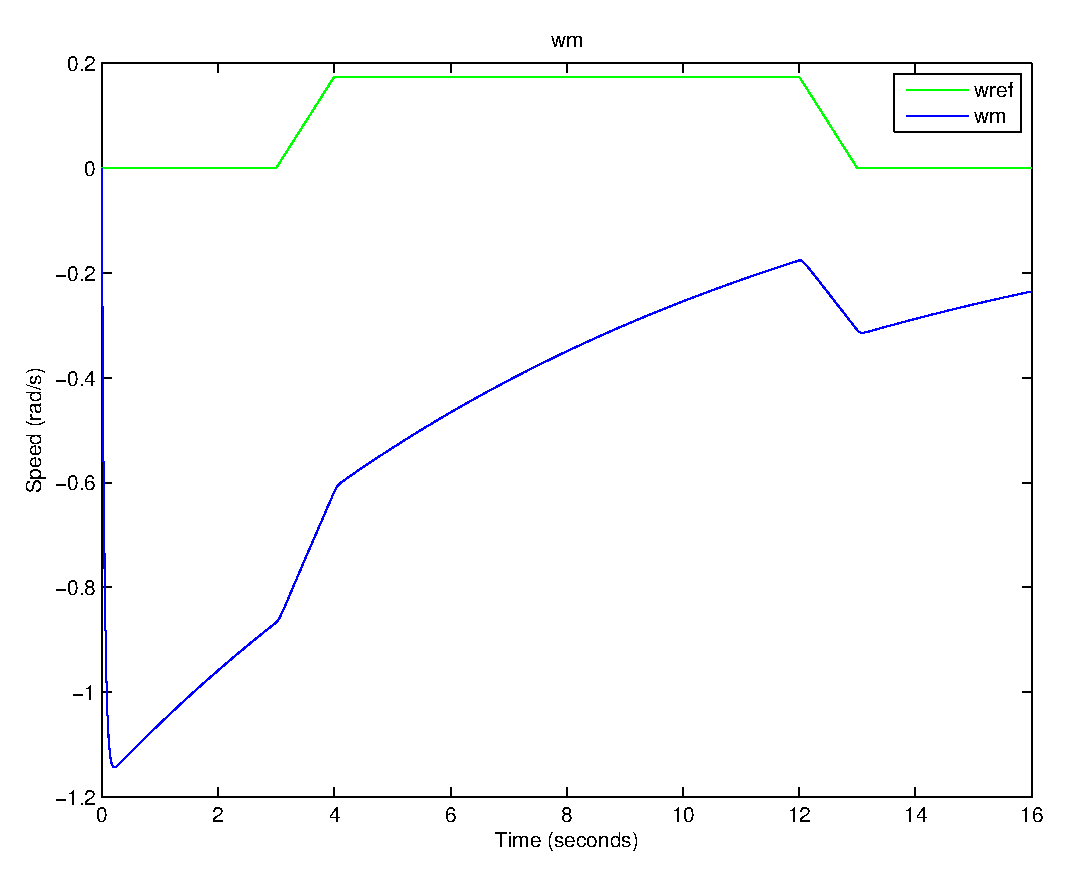
\includegraphics[width=\linewidth]{matlab/wm9}
		\caption{Velocidade angular}
	\end{subfigure}
	\caption{Resposta à perfil de velocidade trapezoidal de 10 segundos}	
	\label{fig:sim9res}
\end{figure}

Como podemos ver o erro estacionário de nosso controlador aumentou drasticamente, isso pois ele foi projetado na situação em que está sem carga. Notamos que embora o perfil de velocidade seja negativo, a posição $\theta$ não fica menor que $0$, isso acontece pois impomos um limite físico ao sistema. As curvas de velocidade requisitadas são muito menores do que a velocidade nominal do motor, explicando o desempenho pobre.

\section{Acoplamento Motor-Robô e Integração do sistema}
Para aumentar o perfil de velocidades requisitado do motor e trabalhar dentro da faixa ideal para nosso servo-controlador, acoplamos o motor e o robô com uma transmissão que reduz a velocidade angular por um fator de 20 vezes. Adicionamos também um controlador P para a posição do robô de ganho proporcional $k_p = 200$. O esquema final do sistema pode ser visto na figura \ref{fig:sim4}.

\begin{figure}[H]
	\centering
	\includegraphics[width=\linewidth]{matlab/sim4}
	\caption{Esquemático da simulação do sistema completo}
	\label{fig:sim4}
\end{figure}

Requisitamos o mesmo perfil de velocidade trapezoidal para a ferramenta, indo de $0$ à $90^\circ$ em 10 segundos, os resultados da simulação são apresentados na figura \ref{fig:sim4res}

\begin{figure}[H]
	\centering
	\begin{subfigure}{0.3\textwidth}
		\includegraphics[width=\linewidth]{matlab/theta4}
		\caption{Posição $\theta$}
	\end{subfigure}
	\begin{subfigure}{0.3\textwidth}
		\includegraphics[width=\linewidth]{matlab/y4}
		\caption{Posição Y}
	\end{subfigure}
	\begin{subfigure}{0.3\textwidth}
		\includegraphics[width=\linewidth]{matlab/x4}
		\caption{Posição X}
	\end{subfigure}
	\begin{subfigure}{0.3\textwidth}
		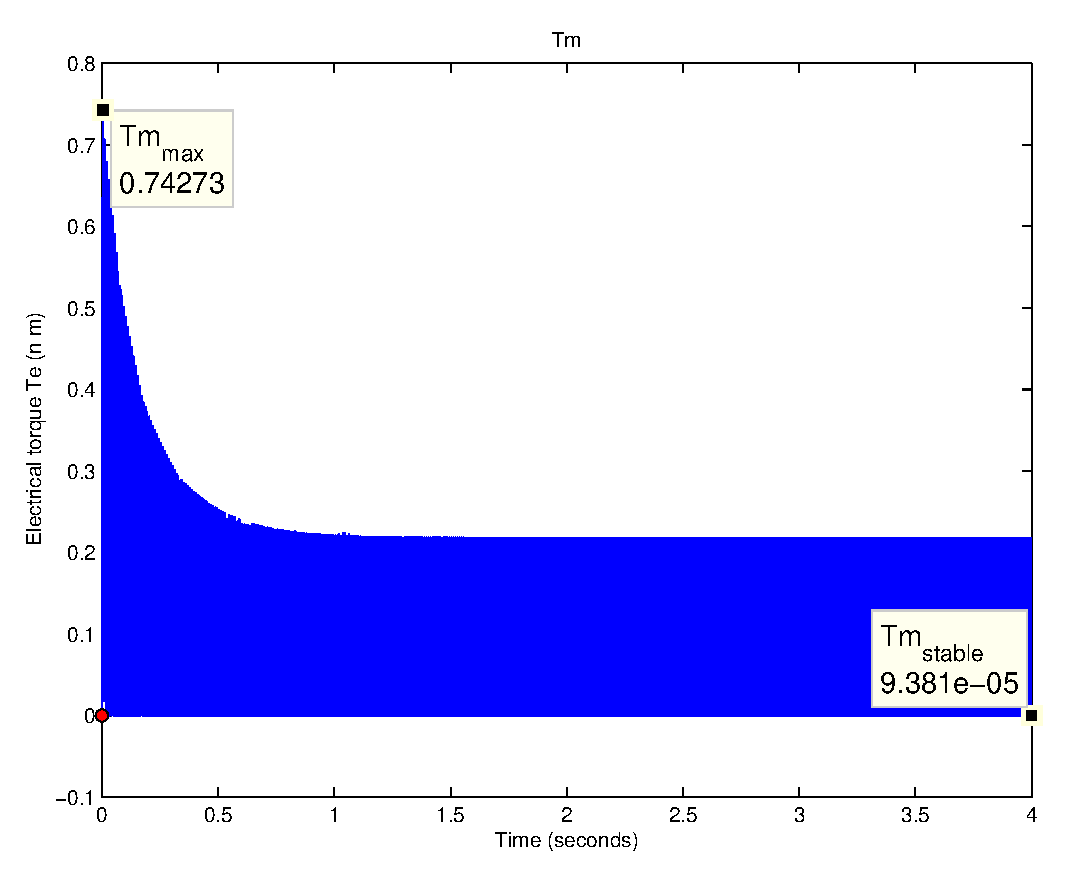
\includegraphics[width=\linewidth]{matlab/tm4}
		\caption{Torque do motor}
	\end{subfigure}
	\begin{subfigure}{0.3\textwidth}
		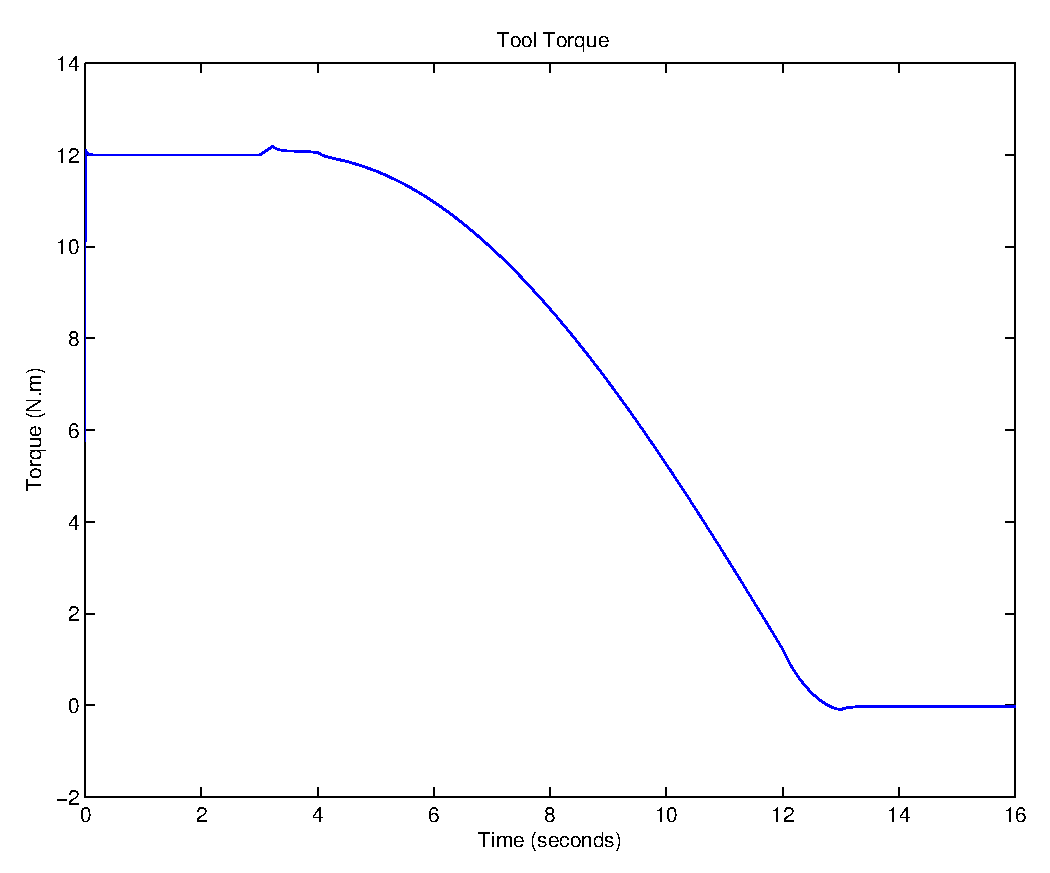
\includegraphics[width=\linewidth]{matlab/t4}
		\caption{Torque da ferramenta}
	\end{subfigure}
	\begin{subfigure}{0.3\textwidth}
		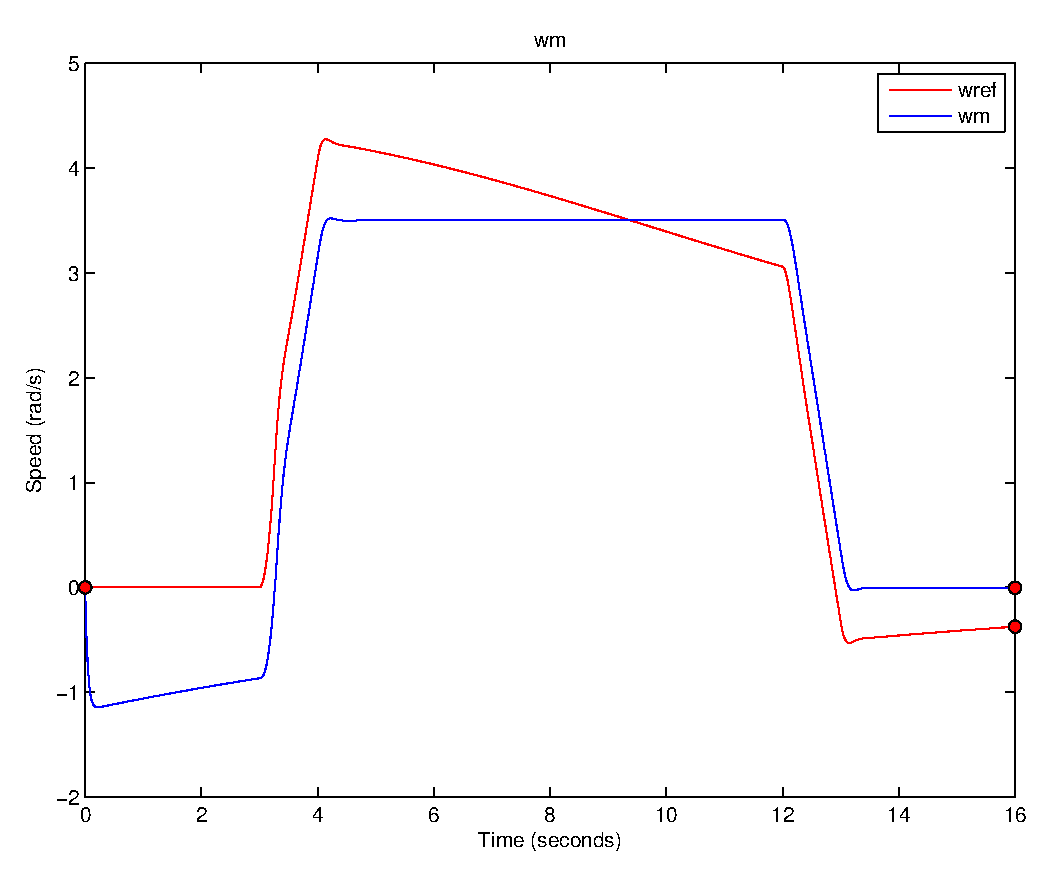
\includegraphics[width=\linewidth]{matlab/wm4}
		\caption{Velocidade angular do motor}
	\end{subfigure}
	\begin{subfigure}{0.3\textwidth}
		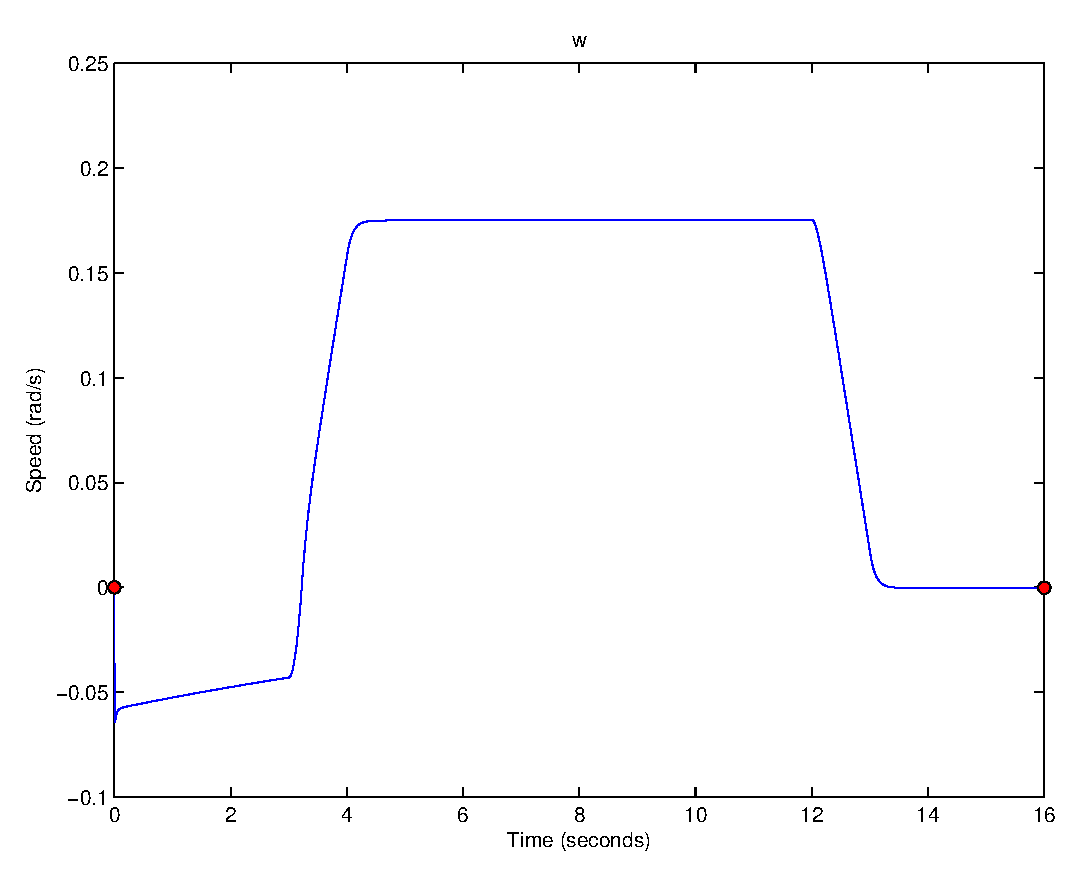
\includegraphics[width=\linewidth]{matlab/w4}
		\caption{Velocidade angular da ferramenta}
	\end{subfigure}
	\begin{subfigure}{0.3\textwidth}
		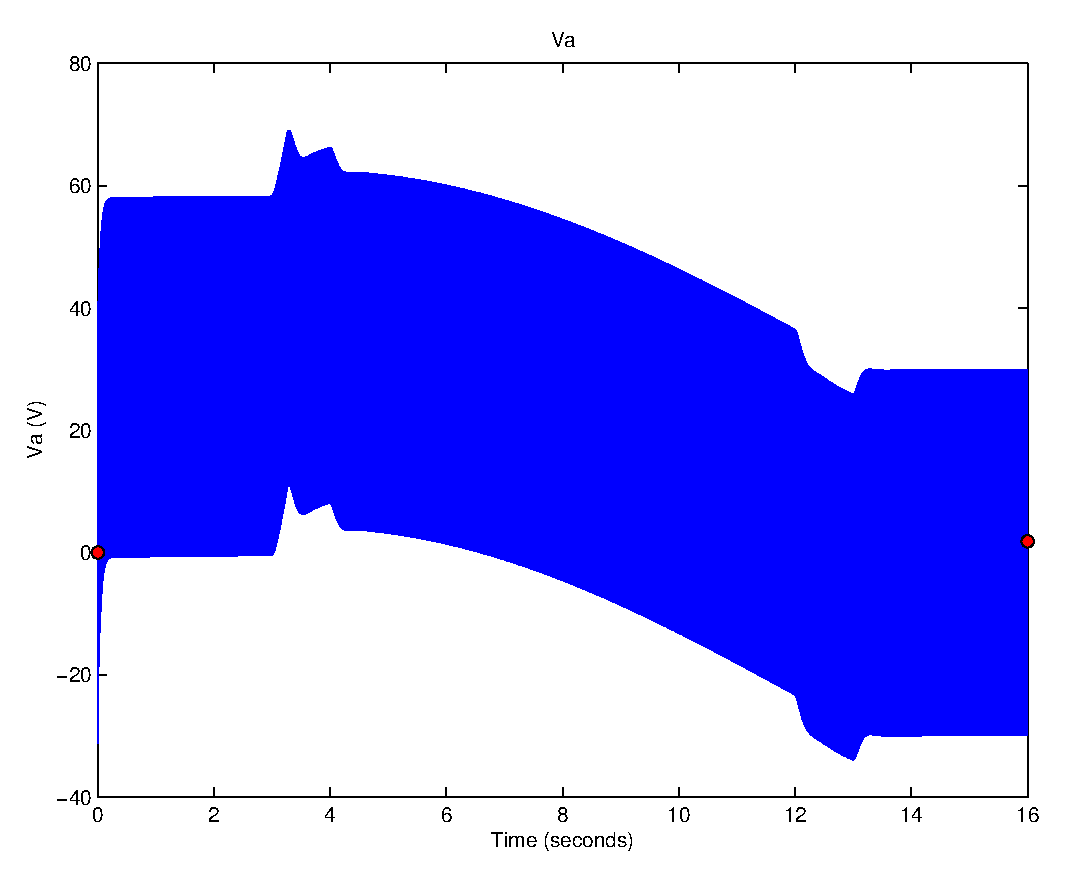
\includegraphics[width=\linewidth]{matlab/va4}
		\caption{Tensão de armadura}
	\end{subfigure}
	\begin{subfigure}{0.3\textwidth}
		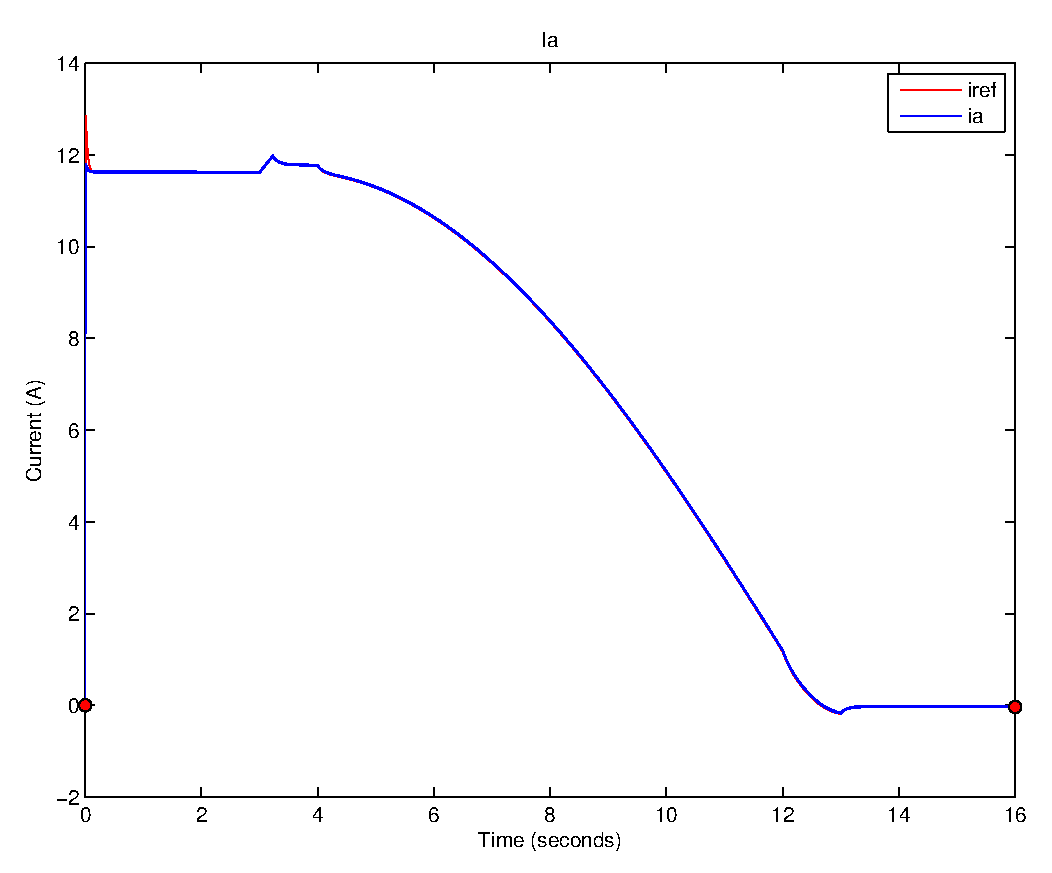
\includegraphics[width=\linewidth]{matlab/ia4}
		\caption{Corrente de armadura}
	\end{subfigure}
	\begin{subfigure}{0.3\textwidth}
		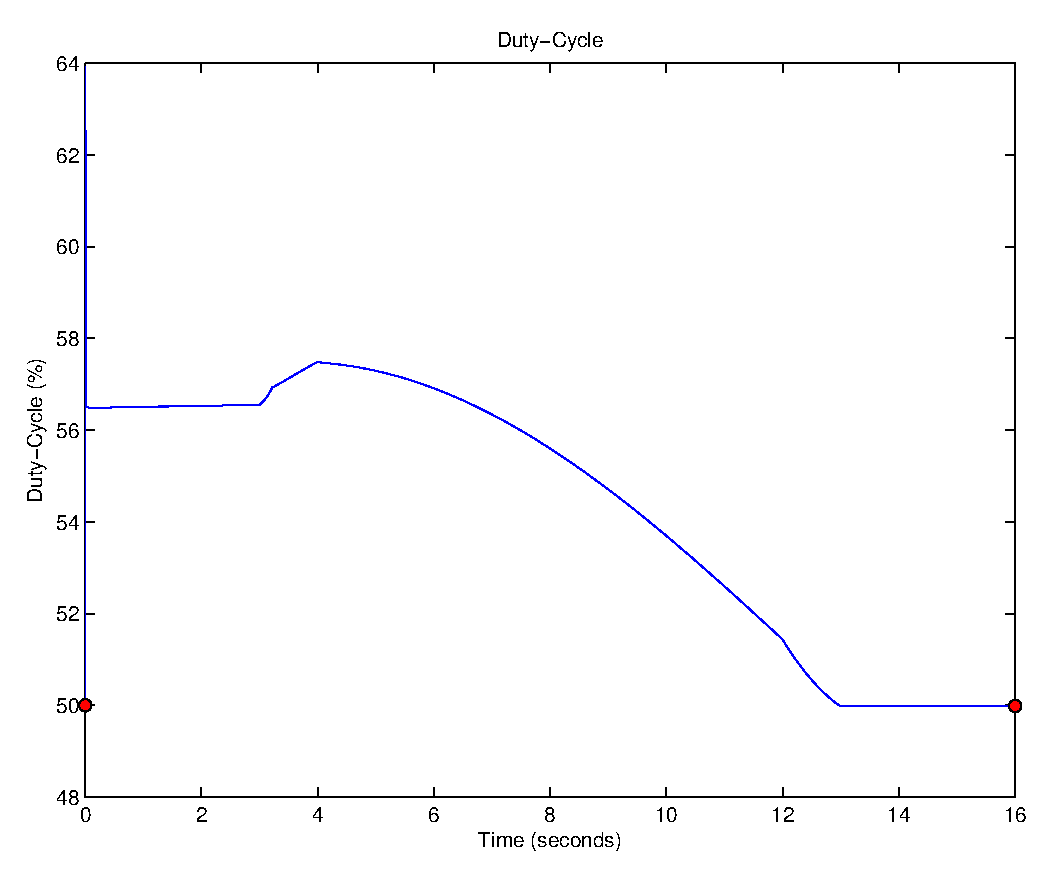
\includegraphics[width=\linewidth]{matlab/d4}
		\caption{Duty-Cycle}
	\end{subfigure}
	\begin{subfigure}{0.3\textwidth}
		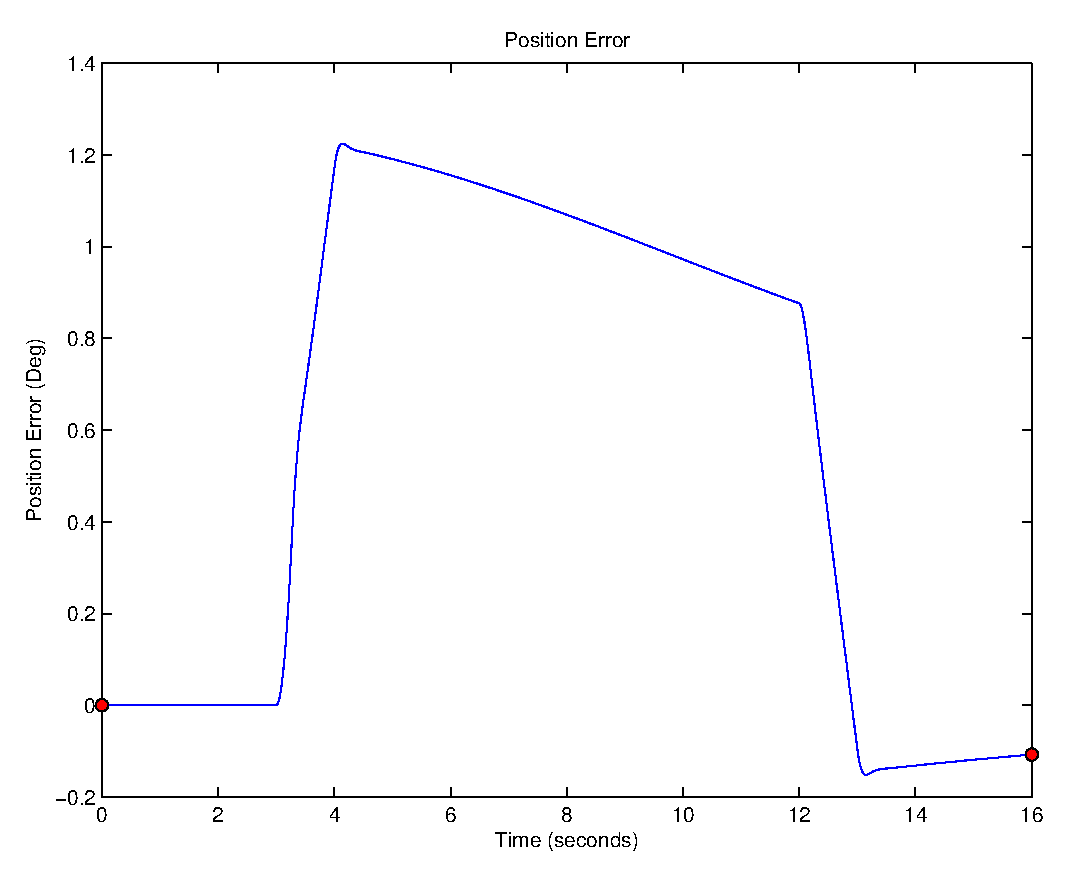
\includegraphics[width=\linewidth]{matlab/ep4}
		\caption{Erro de posição}
	\end{subfigure}
	\begin{subfigure}{0.3\textwidth}
		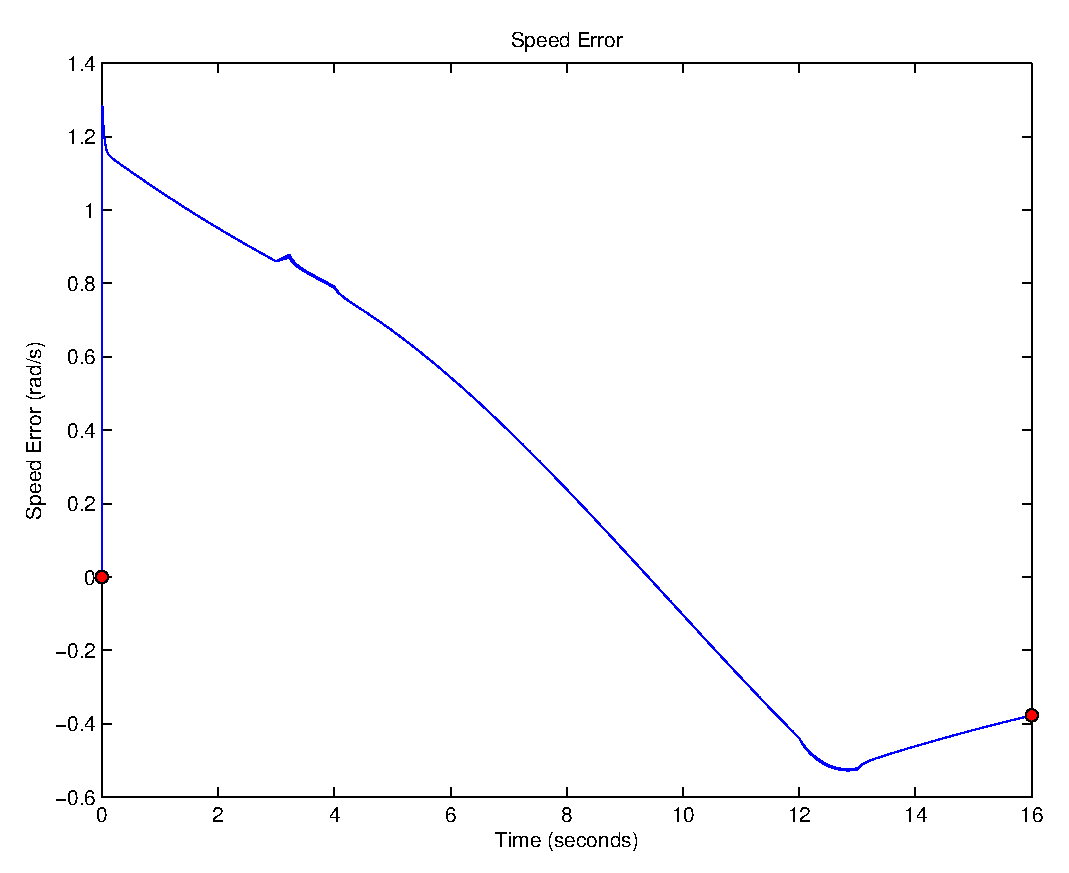
\includegraphics[width=\linewidth]{matlab/ew4}
		\caption{Erro de velocidade}
	\end{subfigure}
	\caption{Resposta à perfil de velocidade trapezoidal de 10 segundos}	
	\label{fig:sim4res}
\end{figure}

Como podemos ver o sistema segue satisfatoriamente a curva desejada. O efeito da carga acoplada distorceu nossa curva de velocidade de referência, uma vez que o torque da posição inicial faz com que o motor adquira uma velocidade negativa, mas o controle em posição foi suficiente para corrigir esse erro.

Simulamos também a resposta do sistema à um perfil de velocidades trapezoidal que leva. o motor da posição $0$ à $70^\circ$ em 5 segundos e depois volta para posição $30^\circ$ em mais 5 e a passos de $10^\circ$ em $10^\circ$ que levam o robô da posição $0$ à $90^\circ$, pausando por dois segundos em cada posição intermediária. As respostas estão apresentadas nas figuras \ref{fig:sim5res} e \ref{fig:sim6res} respectivamente.

\begin{figure}[H]
	\centering
	\begin{subfigure}{0.3\textwidth}
		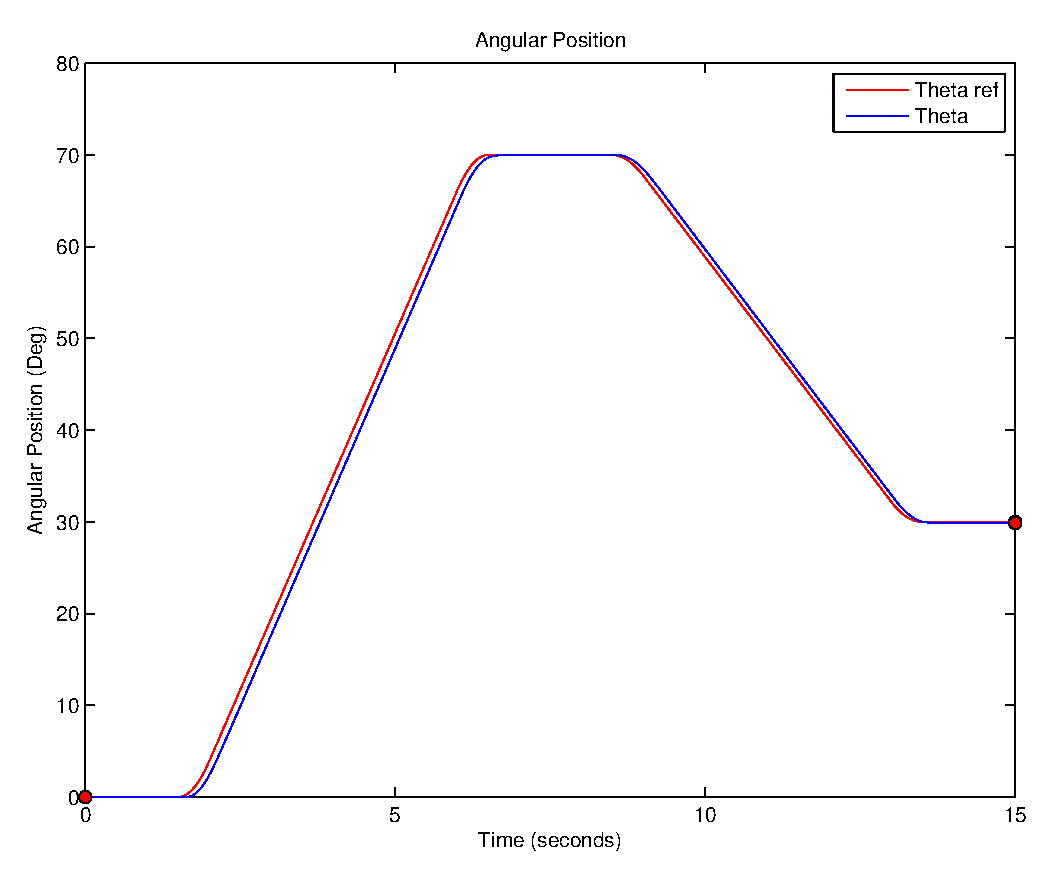
\includegraphics[width=\linewidth]{matlab/theta5}
		\caption{Posição $\theta$}
	\end{subfigure}
	\begin{subfigure}{0.3\textwidth}
		\includegraphics[width=\linewidth]{matlab/y5}
		\caption{Posição Y}
	\end{subfigure}
	\begin{subfigure}{0.3\textwidth}
		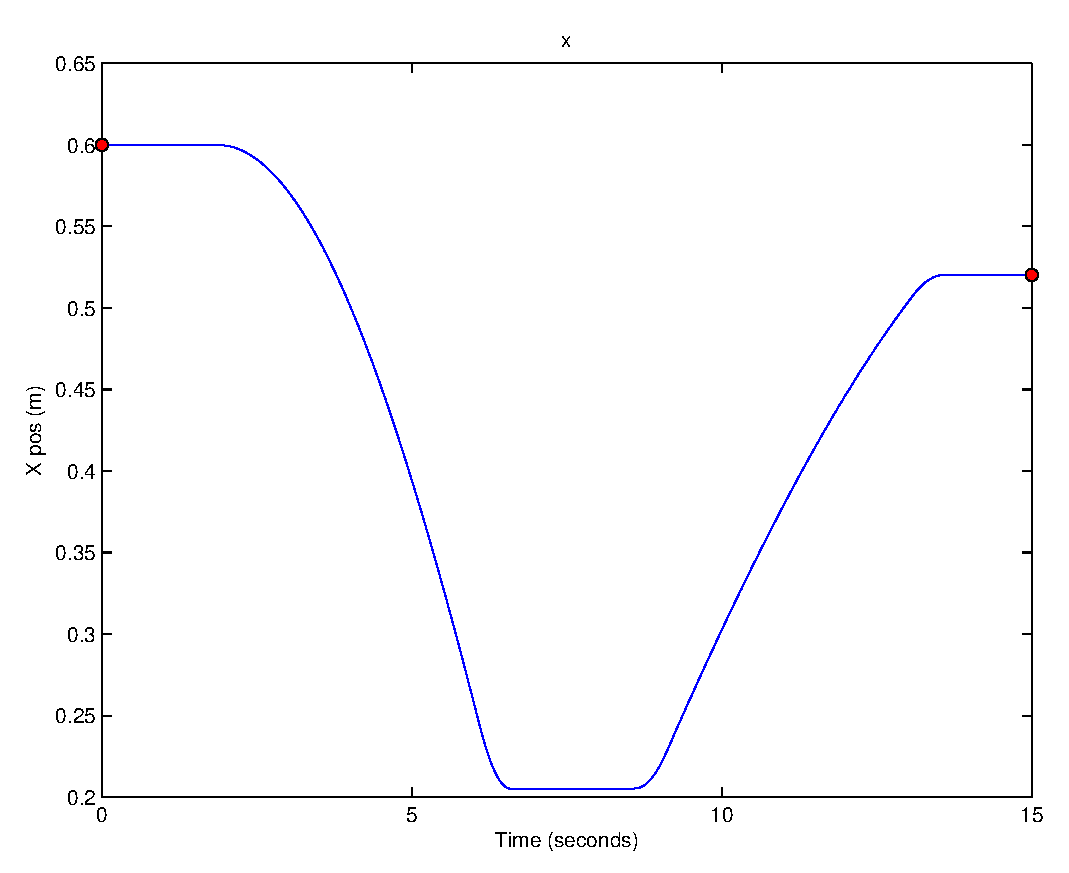
\includegraphics[width=\linewidth]{matlab/x5}
		\caption{Posição X}
	\end{subfigure}
	\begin{subfigure}{0.3\textwidth}
		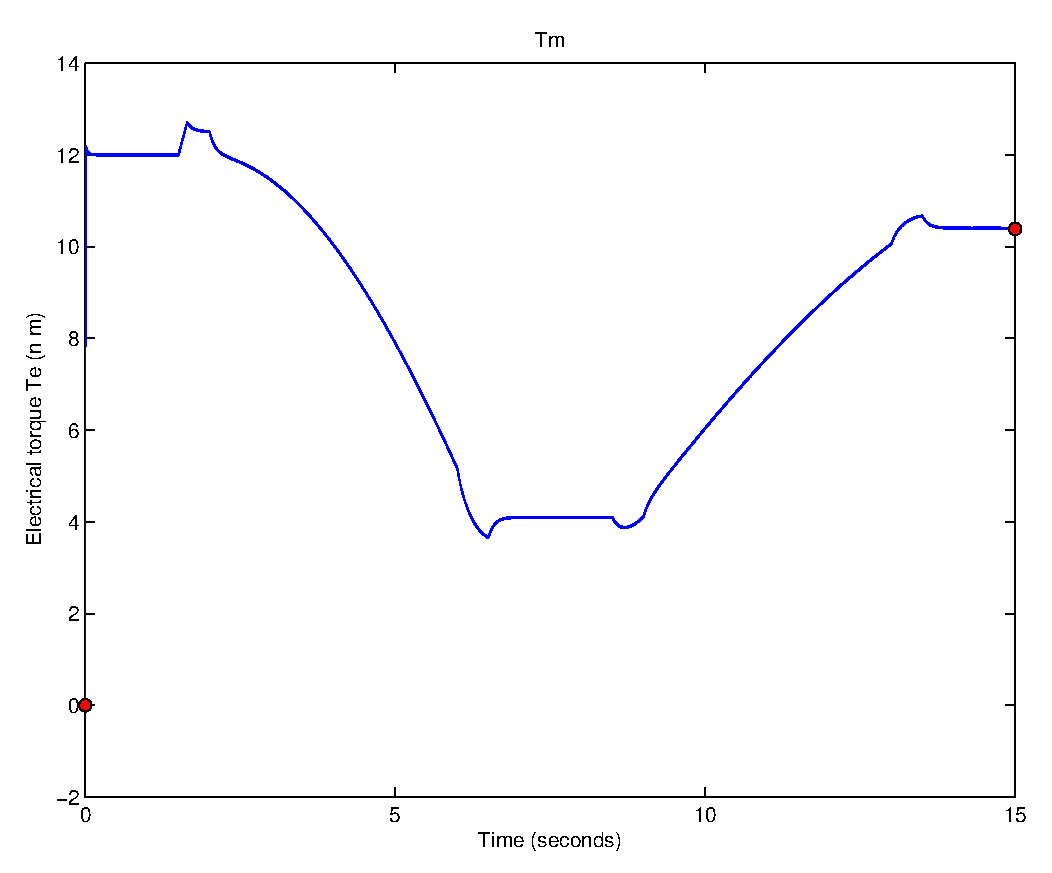
\includegraphics[width=\linewidth]{matlab/tm5}
		\caption{Torque do motor}
	\end{subfigure}
	\begin{subfigure}{0.3\textwidth}
		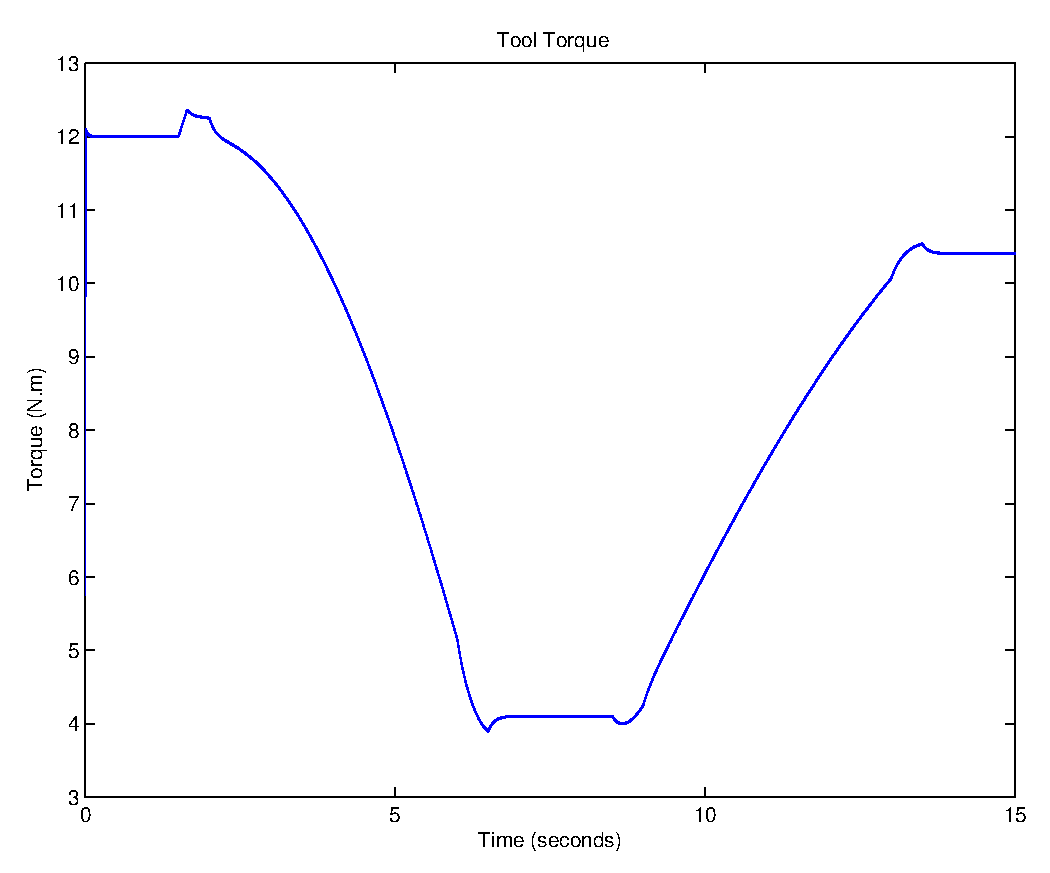
\includegraphics[width=\linewidth]{matlab/t5}
		\caption{Torque da ferramenta}
	\end{subfigure}
	\begin{subfigure}{0.3\textwidth}
		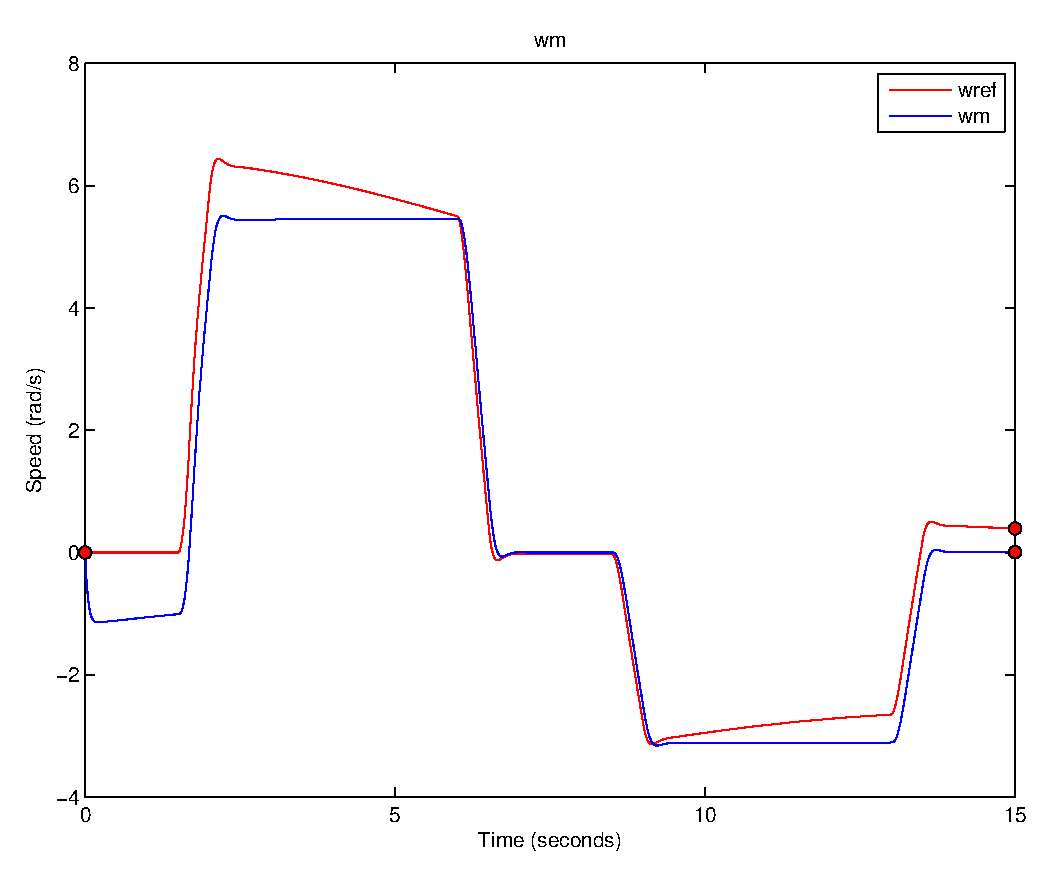
\includegraphics[width=\linewidth]{matlab/wm5}
		\caption{Velocidade angular do motor}
	\end{subfigure}
	\begin{subfigure}{0.3\textwidth}
		\includegraphics[width=\linewidth]{matlab/w5}
		\caption{Velocidade angular da ferramenta}
	\end{subfigure}
	\begin{subfigure}{0.3\textwidth}
		\includegraphics[width=\linewidth]{matlab/va5}
		\caption{Tensão de armadura}
	\end{subfigure}
	\begin{subfigure}{0.3\textwidth}
		\includegraphics[width=\linewidth]{matlab/ia5}
		\caption{Corrente de armadura}
	\end{subfigure}
	\begin{subfigure}{0.3\textwidth}
		\includegraphics[width=\linewidth]{matlab/d5}
		\caption{Duty-Cycle}
	\end{subfigure}
	\begin{subfigure}{0.3\textwidth}
		\includegraphics[width=\linewidth]{matlab/ep5}
		\caption{Erro de posição}
	\end{subfigure}
	\begin{subfigure}{0.3\textwidth}
		\includegraphics[width=\linewidth]{matlab/ew5}
		\caption{Erro de velocidade}
	\end{subfigure}
	\caption{Resposta à perfil de velocidade trapezoidal com ida e volta em 5 segundos cada}	
	\label{fig:sim5res}
\end{figure}

\begin{figure}[H]
	\centering
	\begin{subfigure}{0.3\textwidth}
		\includegraphics[width=\linewidth]{matlab/theta6}
		\caption{Posição $\theta$}
	\end{subfigure}
	\begin{subfigure}{0.3\textwidth}
		\includegraphics[width=\linewidth]{matlab/y6}
		\caption{Posição Y}
	\end{subfigure}
	\begin{subfigure}{0.3\textwidth}
		\includegraphics[width=\linewidth]{matlab/x6}
		\caption{Posição X}
	\end{subfigure}
	\begin{subfigure}{0.3\textwidth}
		\includegraphics[width=\linewidth]{matlab/tm6}
		\caption{Torque do motor}
	\end{subfigure}
	\begin{subfigure}{0.3\textwidth}
		\includegraphics[width=\linewidth]{matlab/t6}
		\caption{Torque da ferramenta}
	\end{subfigure}
	\begin{subfigure}{0.3\textwidth}
		\includegraphics[width=\linewidth]{matlab/wm6}
		\caption{Velocidade angular do motor}
	\end{subfigure}
	\begin{subfigure}{0.3\textwidth}
		\includegraphics[width=\linewidth]{matlab/w6}
		\caption{Velocidade angular da ferramenta}
	\end{subfigure}
	\begin{subfigure}{0.3\textwidth}
		\includegraphics[width=\linewidth]{matlab/va6}
		\caption{Tensão de armadura}
	\end{subfigure}
	\begin{subfigure}{0.3\textwidth}
		\includegraphics[width=\linewidth]{matlab/ia6}
		\caption{Corrente de armadura}
	\end{subfigure}
	\begin{subfigure}{0.3\textwidth}
		\includegraphics[width=\linewidth]{matlab/d6}
		\caption{Duty-Cycle}
	\end{subfigure}
	\begin{subfigure}{0.3\textwidth}
		\includegraphics[width=\linewidth]{matlab/ep6}
		\caption{Erro de posição}
	\end{subfigure}
	\begin{subfigure}{0.3\textwidth}
		\includegraphics[width=\linewidth]{matlab/ew6}
		\caption{Erro de velocidade}
	\end{subfigure}
	\caption{Resposta à degraus de posição}	
	\label{fig:sim6res}
\end{figure}

\bibliography{mybib}
\end{document}

